\section{Messung des Emissionsspektrums}
%kurz das ziel dieses versuchsteiles ansprechen, damit keine zwei �berschriften direkt �bereinander stehen!
%bei schwierigeren versuchen kann auch der theoretische hintergrund erl�utert werden. (mit formeln, herleitungen und erkl�rungen)
Im ersten Versuchsteil wird das R�ntgenspektrum der Kupferanode mit einem Silicium(111)-Einkristall untersucht, f�r die Untersuchung werden drei verschieden Beschleunigungsspannungen und ein Ni-Filter verwendet. Untersucht werden die Z�hlraten in Abh�ngigkeit des Winkels, sowie die Lage aller Ordnungen der K$_{\alpha_{1,2}}$- und K$_\beta$-Linien von Kupfer und deren Verh�ltnisse. Dann wird das Signal-Rausch-Verh�ltnis untersucht und weitere Details der Spektren besprochen. Im Anschluss werden die Netzebenabst�nde anderer Einkristalle untersucht. Untersucht werden Si(331)- und Ge(111)-Einkristalle. Die bestimmten Netzebenabst�nde werden mit Literaturwerten abgeglichen.

%Versuchsdurchf�hrung
\section{Versuchsdurchf�hrung}
%erkl�ren, !was! wir machen, !warum! wir das machen und mit welchem ziel
%(wichtig) pr�zize erkl�ren, wie bei dem versuch vorgegangen und was gemacht wurde
\subsection{Hochspannung der Photomultiplier}
Ein exaktes einstellen der Photomulitplier ist ist essenziell f�r eine gute Messung. Die Spannungen von PM1, PM2 und PM4 sollen dabei einen Wert von 2100 V nicht �berschreiten. Der Arbeitspunkt von PM3 liegt im Bereich von 2600-2700 V. F�r die Bestimmung des optimalen Arbeitspunktes wird die Schwelle des Diskriminators auf einen m�glichst geringen Wert eingestellt. Es wird die die Z�hlrate in Abh�ngigkeit der Spannung untersucht und nach einem  Plateau im Bereich von 100 bis 1000 Counts/s gesucht, da sich der Photomulitplier dann am optimalen Arbeitspunkt befindet. Falls die Z�hlraten zu niedrig sind kann ein $^{60}Co$-Pr�parat verwendet werden, um die Z�hlrate zu erh�hen.

Die aufgenommenen Spannungskennlinien sind in Abbildung ?? bis ?? zu sehen.

%Auswertung der Spannungskennlinien, beschreibung der Plots

Die bestimmten Spannungen f�r die Photomulitplier sind in Tabelle \ref{tab:hochspannung} aufgetragen.

\begin{table}[H]
\centering
\caption{Verwendete Spannungen f�r die Photomuliplier}
\label{tab:hochspannung}
\begin{tabular}{|c|c|}
\hline Photomultiplier & Spannung[V] \\ \hline
\hline PM1 &  \\ 
\hline PM2 &  \\ 
\hline PM3 &  \\ 
\hline PM4 &  \\ 
\hline 
\end{tabular} 
\end{table}
\subsection{Schwellspannung}
Mit den Szintillatoren soll minimal ionisierende Strahlung gemessen werden. Daf�r werden die Schwellen etwas unterhalb des Energieverlustes der Flach-Szintillatoren, im Bereich von 1,2MeV eingestellt. F�r die Justierung wird ein $^{60}$Co Pr�parat verwendet. Die untere Schwelle f�r den Blockdiskriminator, im Bereich von 1,5-2MeV soll m�glichst niedrig eingestellt werden, jedoch hoch genug, um den Untergrund der Praktikumsr�ume auszublenden. Dabei soll das Signal-Rausch-Verh�ltnis maximal werden. Um das Signal-Rausch-Verh�ltnis zu maximieren, wurde zuerst bei allen Diskriminatoren die Differenz zwischen dem Signal mit $^{60}$Co-Pr�parat und dem Signal ohne $^{60}$Co-Pr�parat bestimmt. Die bestimmten Schwellspannungen sind in den Abb. \ref{fig:Disk_1}, \ref{fig:Disk_2}, \ref{fig:Disk_3} und \ref{fig:Disk_4} zu sehen.
\begin{figure}[H]
\centering
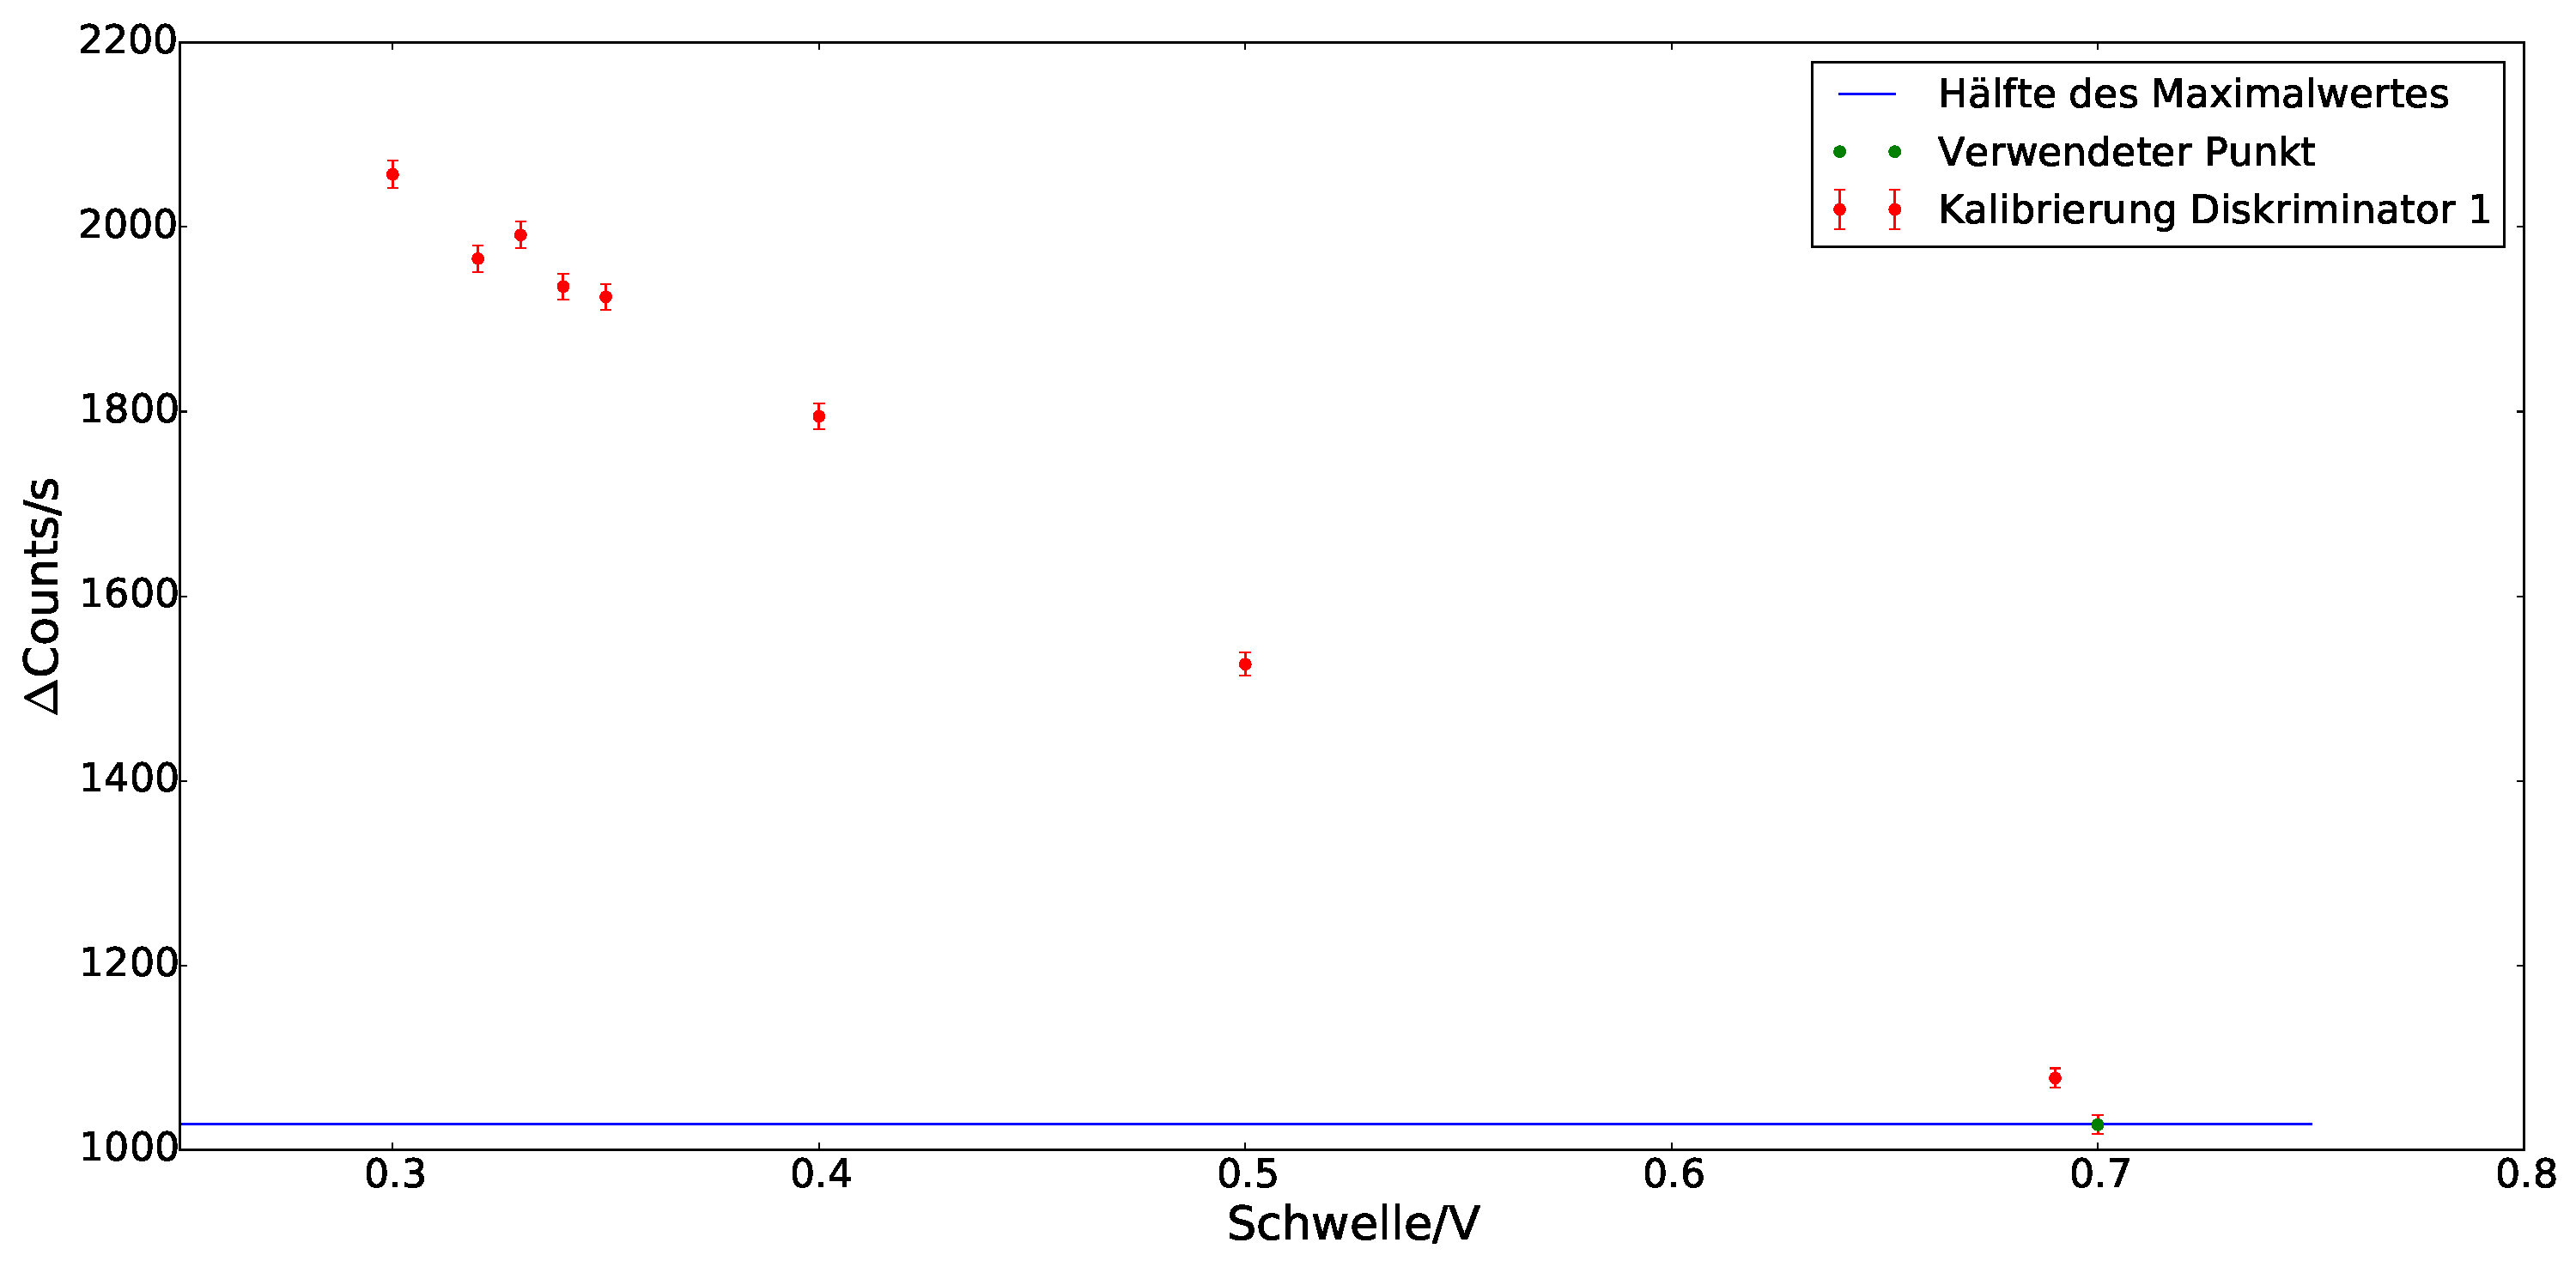
\includegraphics[scale = 0.35]{Disk_1.pdf}
\caption{Differenzplot der Counts gegen die Schwellspannung f�r Diskriminator 1}
\label{fig:Disk_1}
\end{figure}
\begin{figure}[H]
\centering
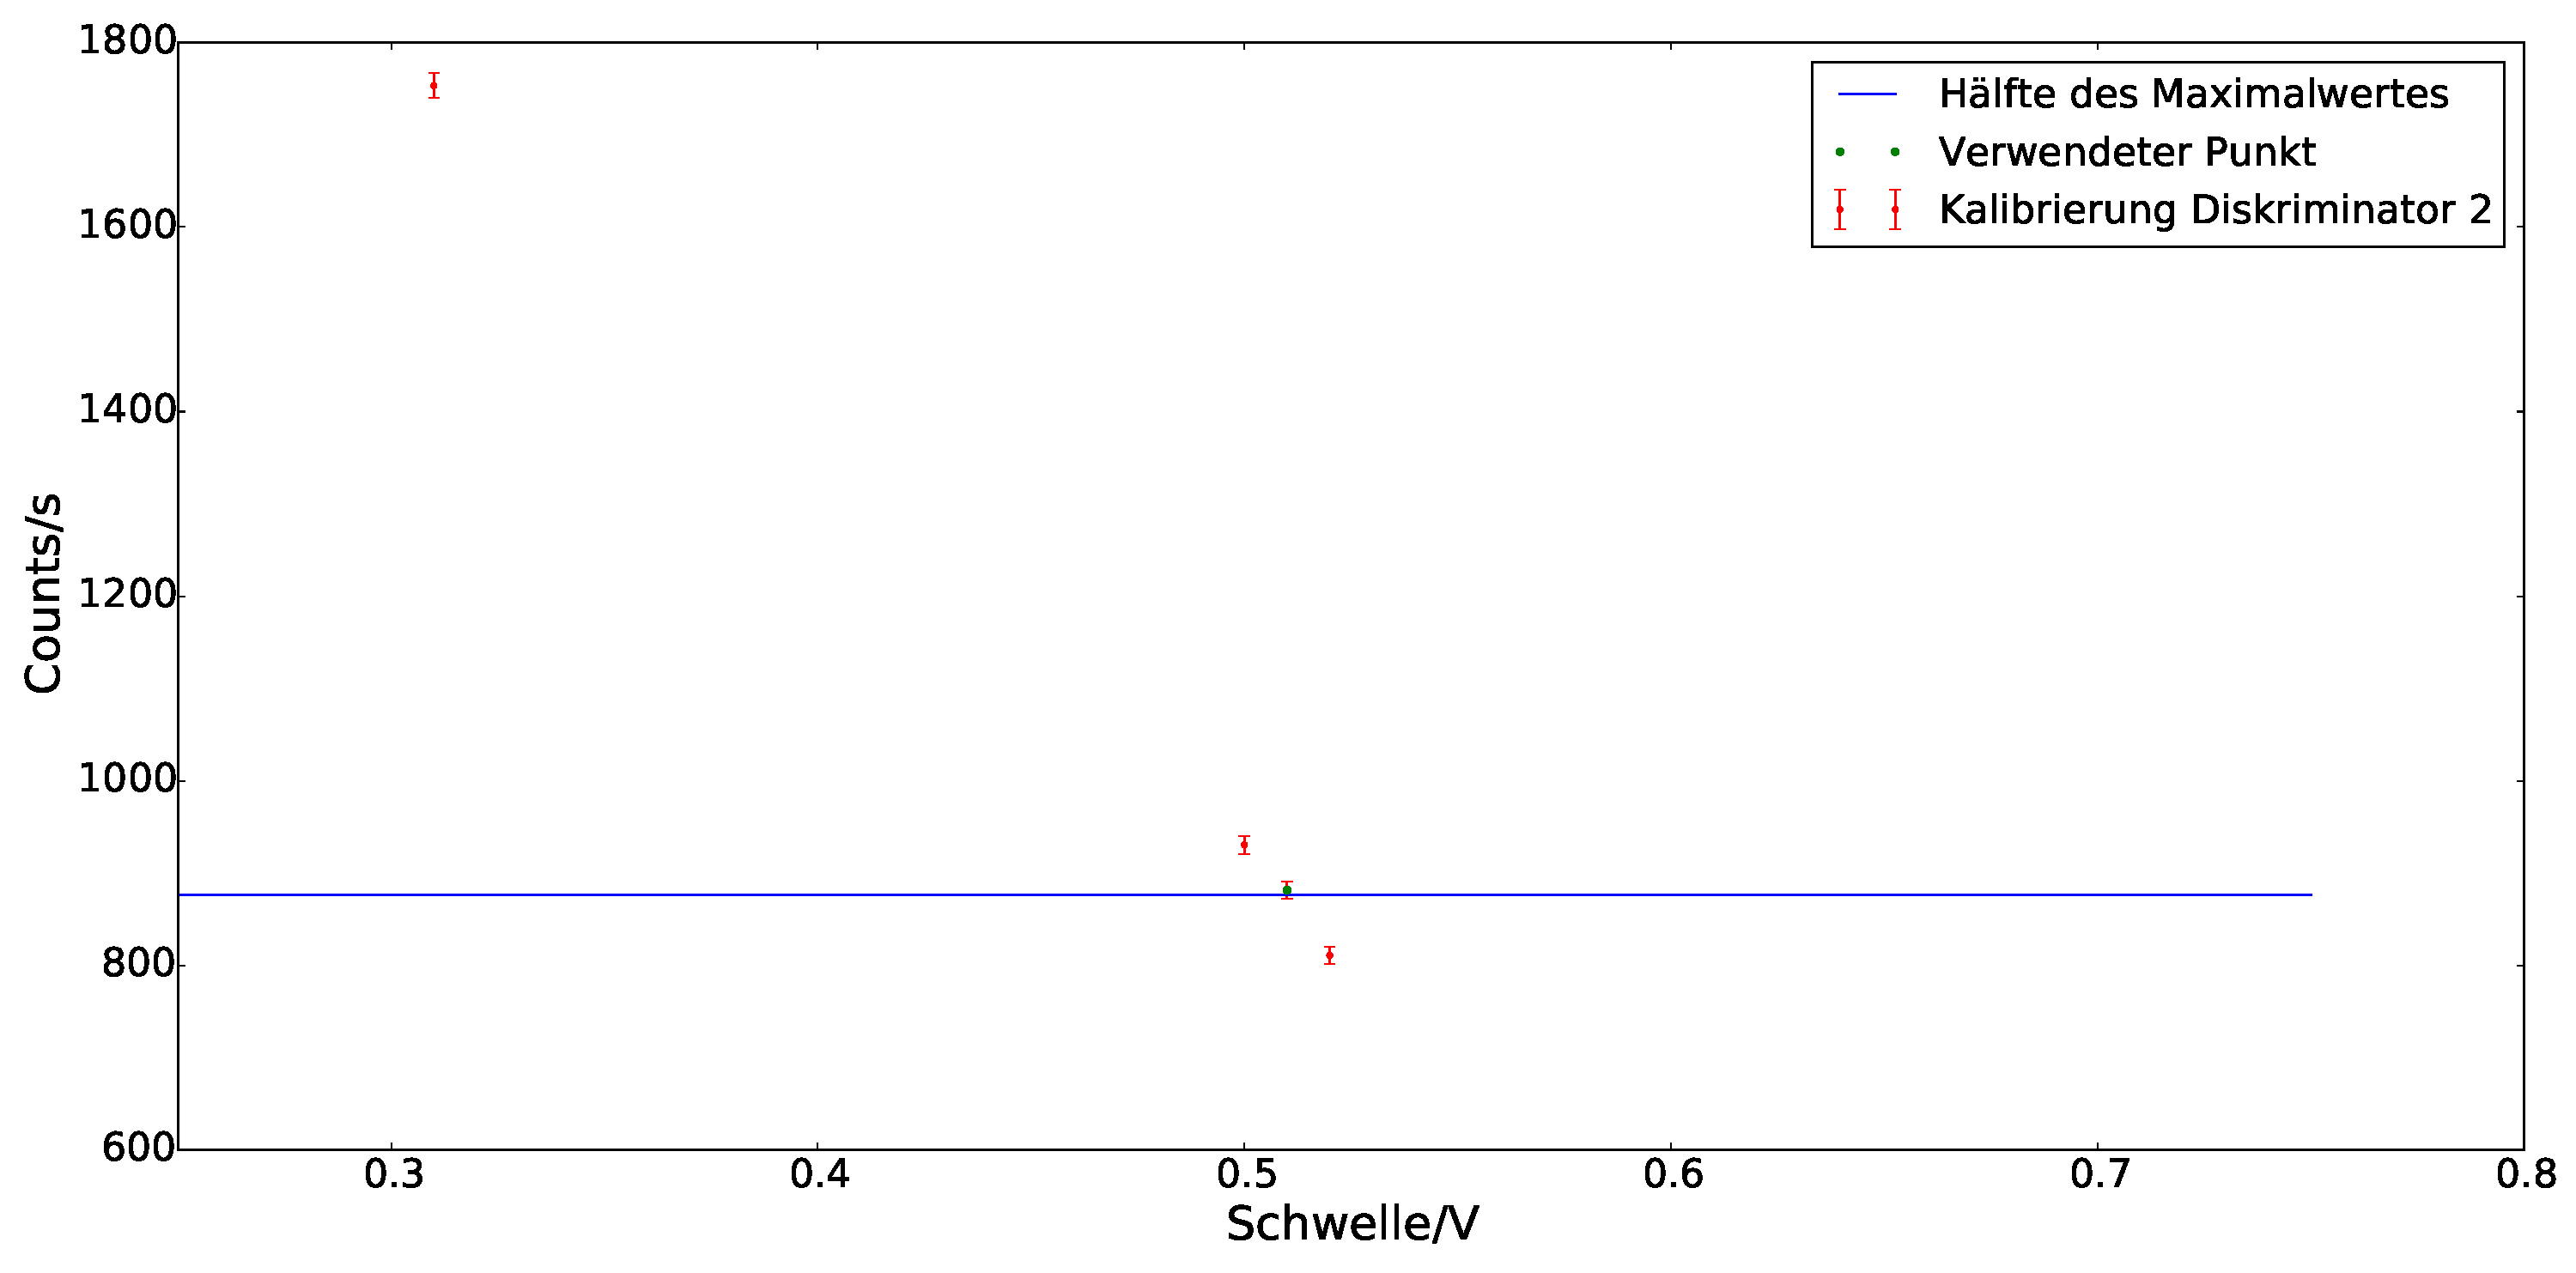
\includegraphics[scale = 0.35]{Disk_2.pdf}
\caption{Differenzplot der Counts gegen die Schwellspannung f�r Diskriminator 2}
\label{fig:Disk_2}
\end{figure}
In Abb. \ref{fig:Disk_3} wurde zus�tzlich eine etwas h�here Schwelle eingestellt, welche auf H�he des Plateaus zwischen den beiden Energien der von $^{60}$Co emittierten Photonen liegt. Nach der Einstellung des Delays, wodurch erreicht werden soll, dass die beiden oberen Szintillatoren (1 und 2) gleichzeitig mit dem 3. Szitillator triggern, wird die Diskriminatorschwelle f�r den 3. Szintillator auf den h�heren Wert gestellt, sodass dieser w�hrend der Messung nur bei Zerfall eines Myons triggert. Szintillator 1 und 2 triggern w�hrend der Messung genau beim Eintritt des Myons in Szintillator 3, wobei Szintillator 3 erst im Falle eines Zerfalls triggert (2. Diskriminatorschwelle). 
\begin{figure}[H]
\centering
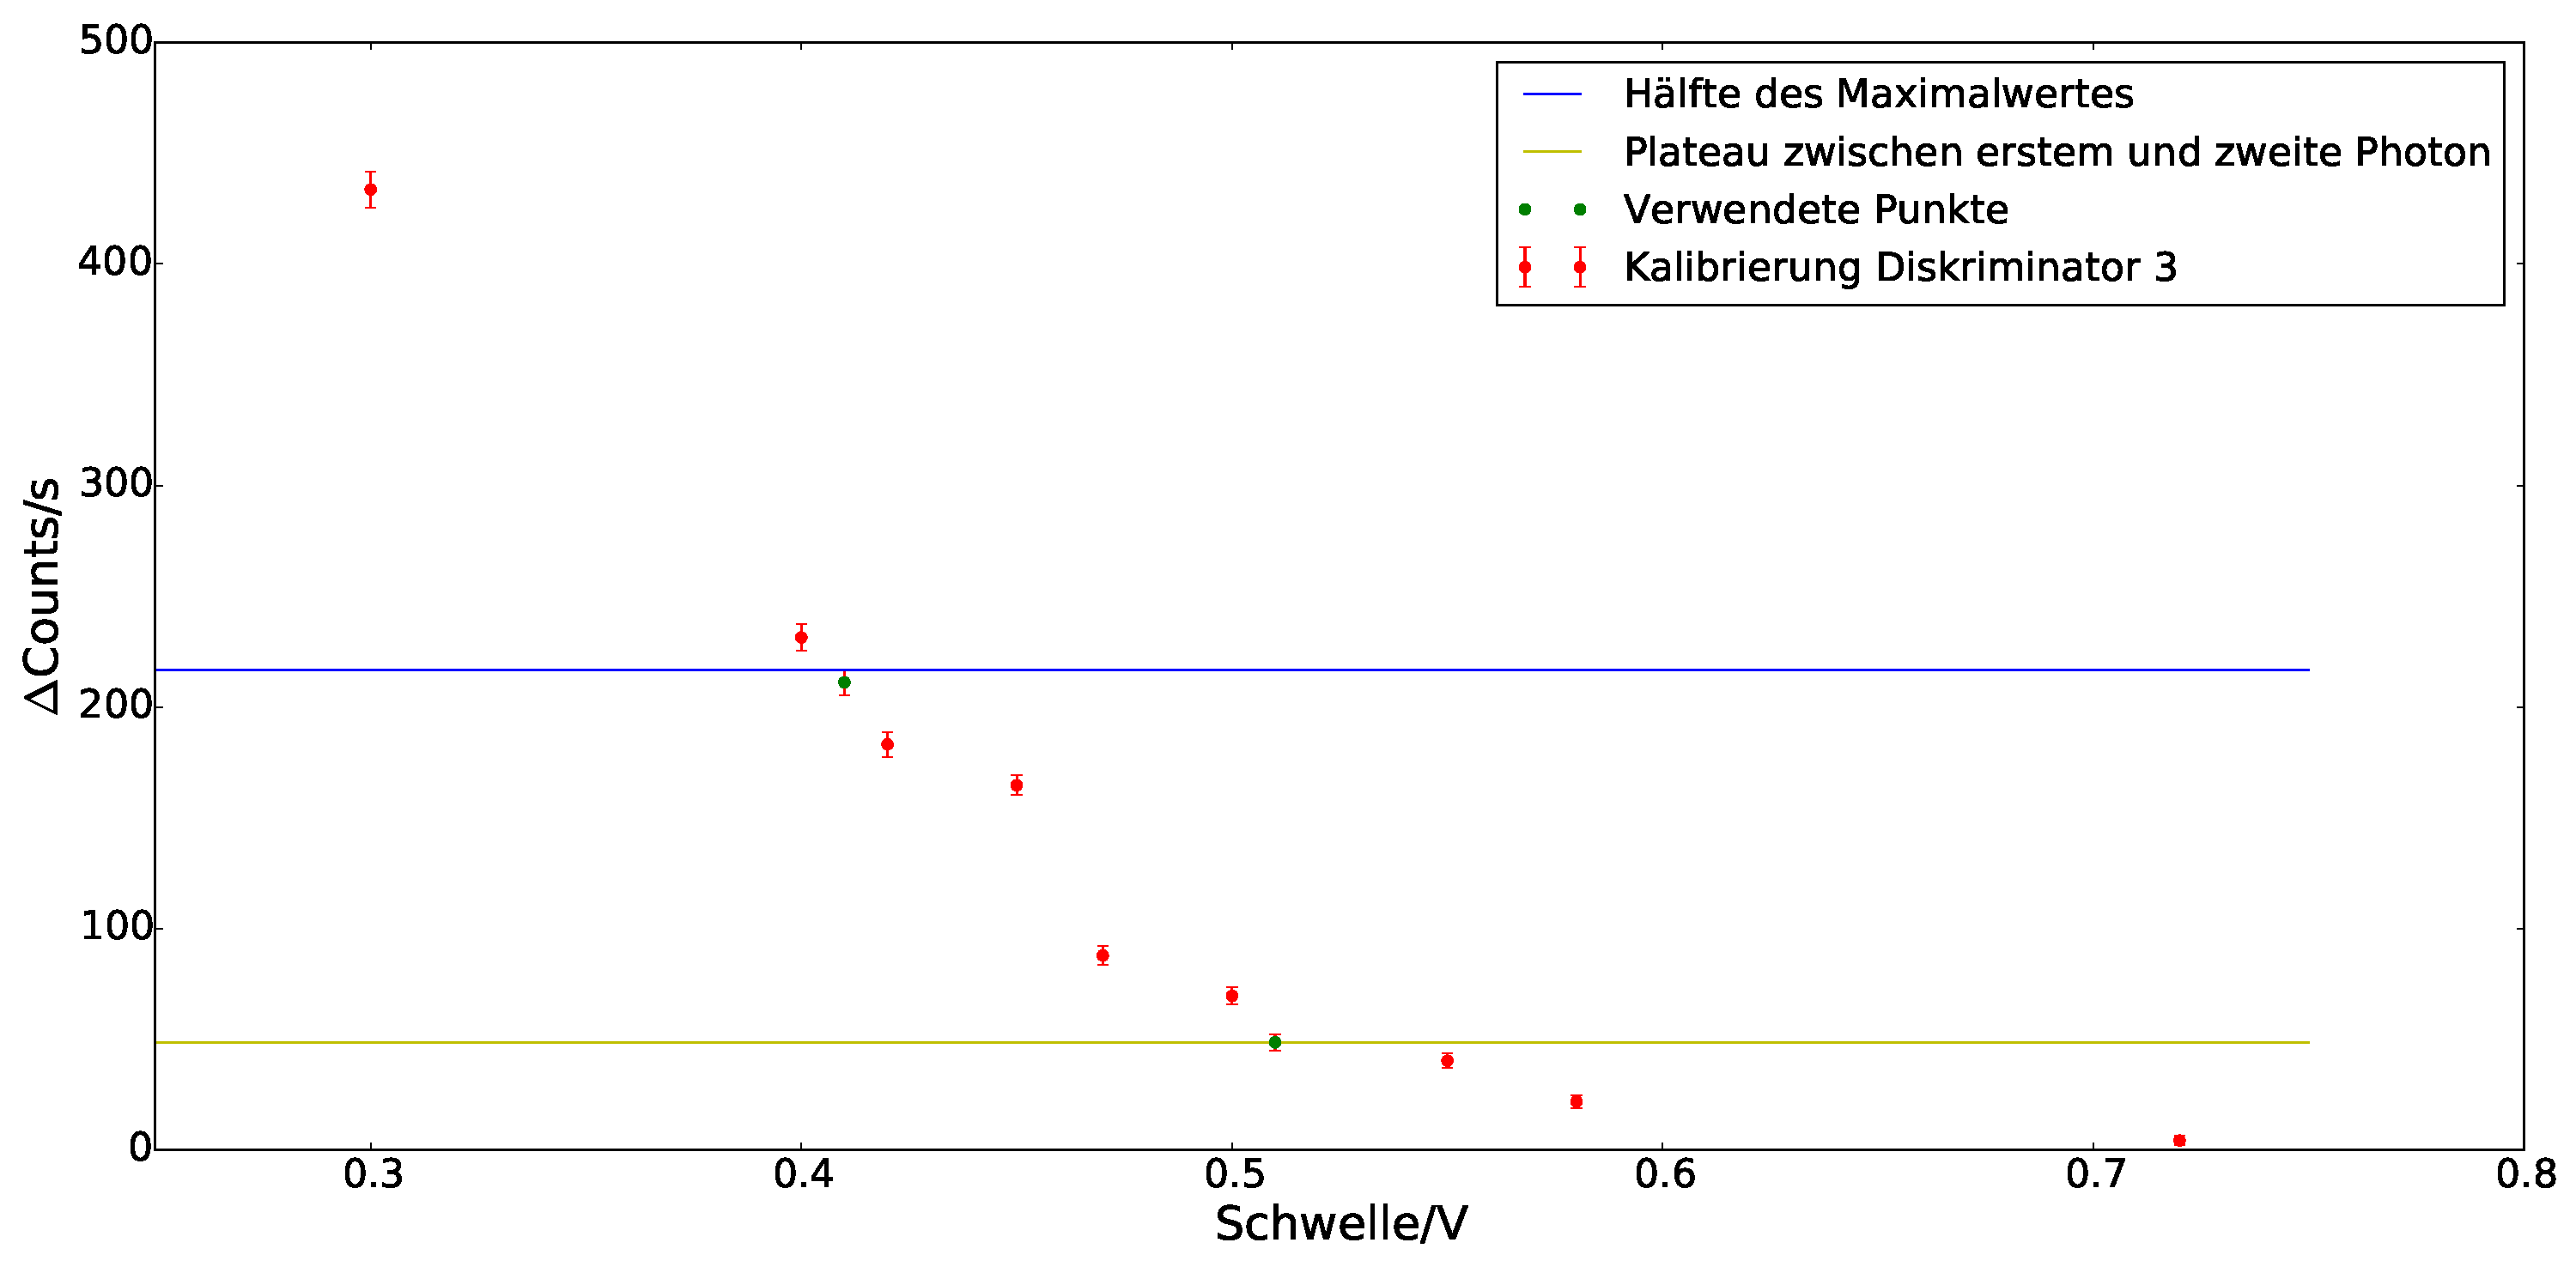
\includegraphics[scale = 0.35]{Disk_3.pdf}
\caption{Differenzplot der Counts gegen die Schwellspannung f�r Diskriminator 3}
\label{fig:Disk_3}
\end{figure}
\begin{figure}[H]
\centering
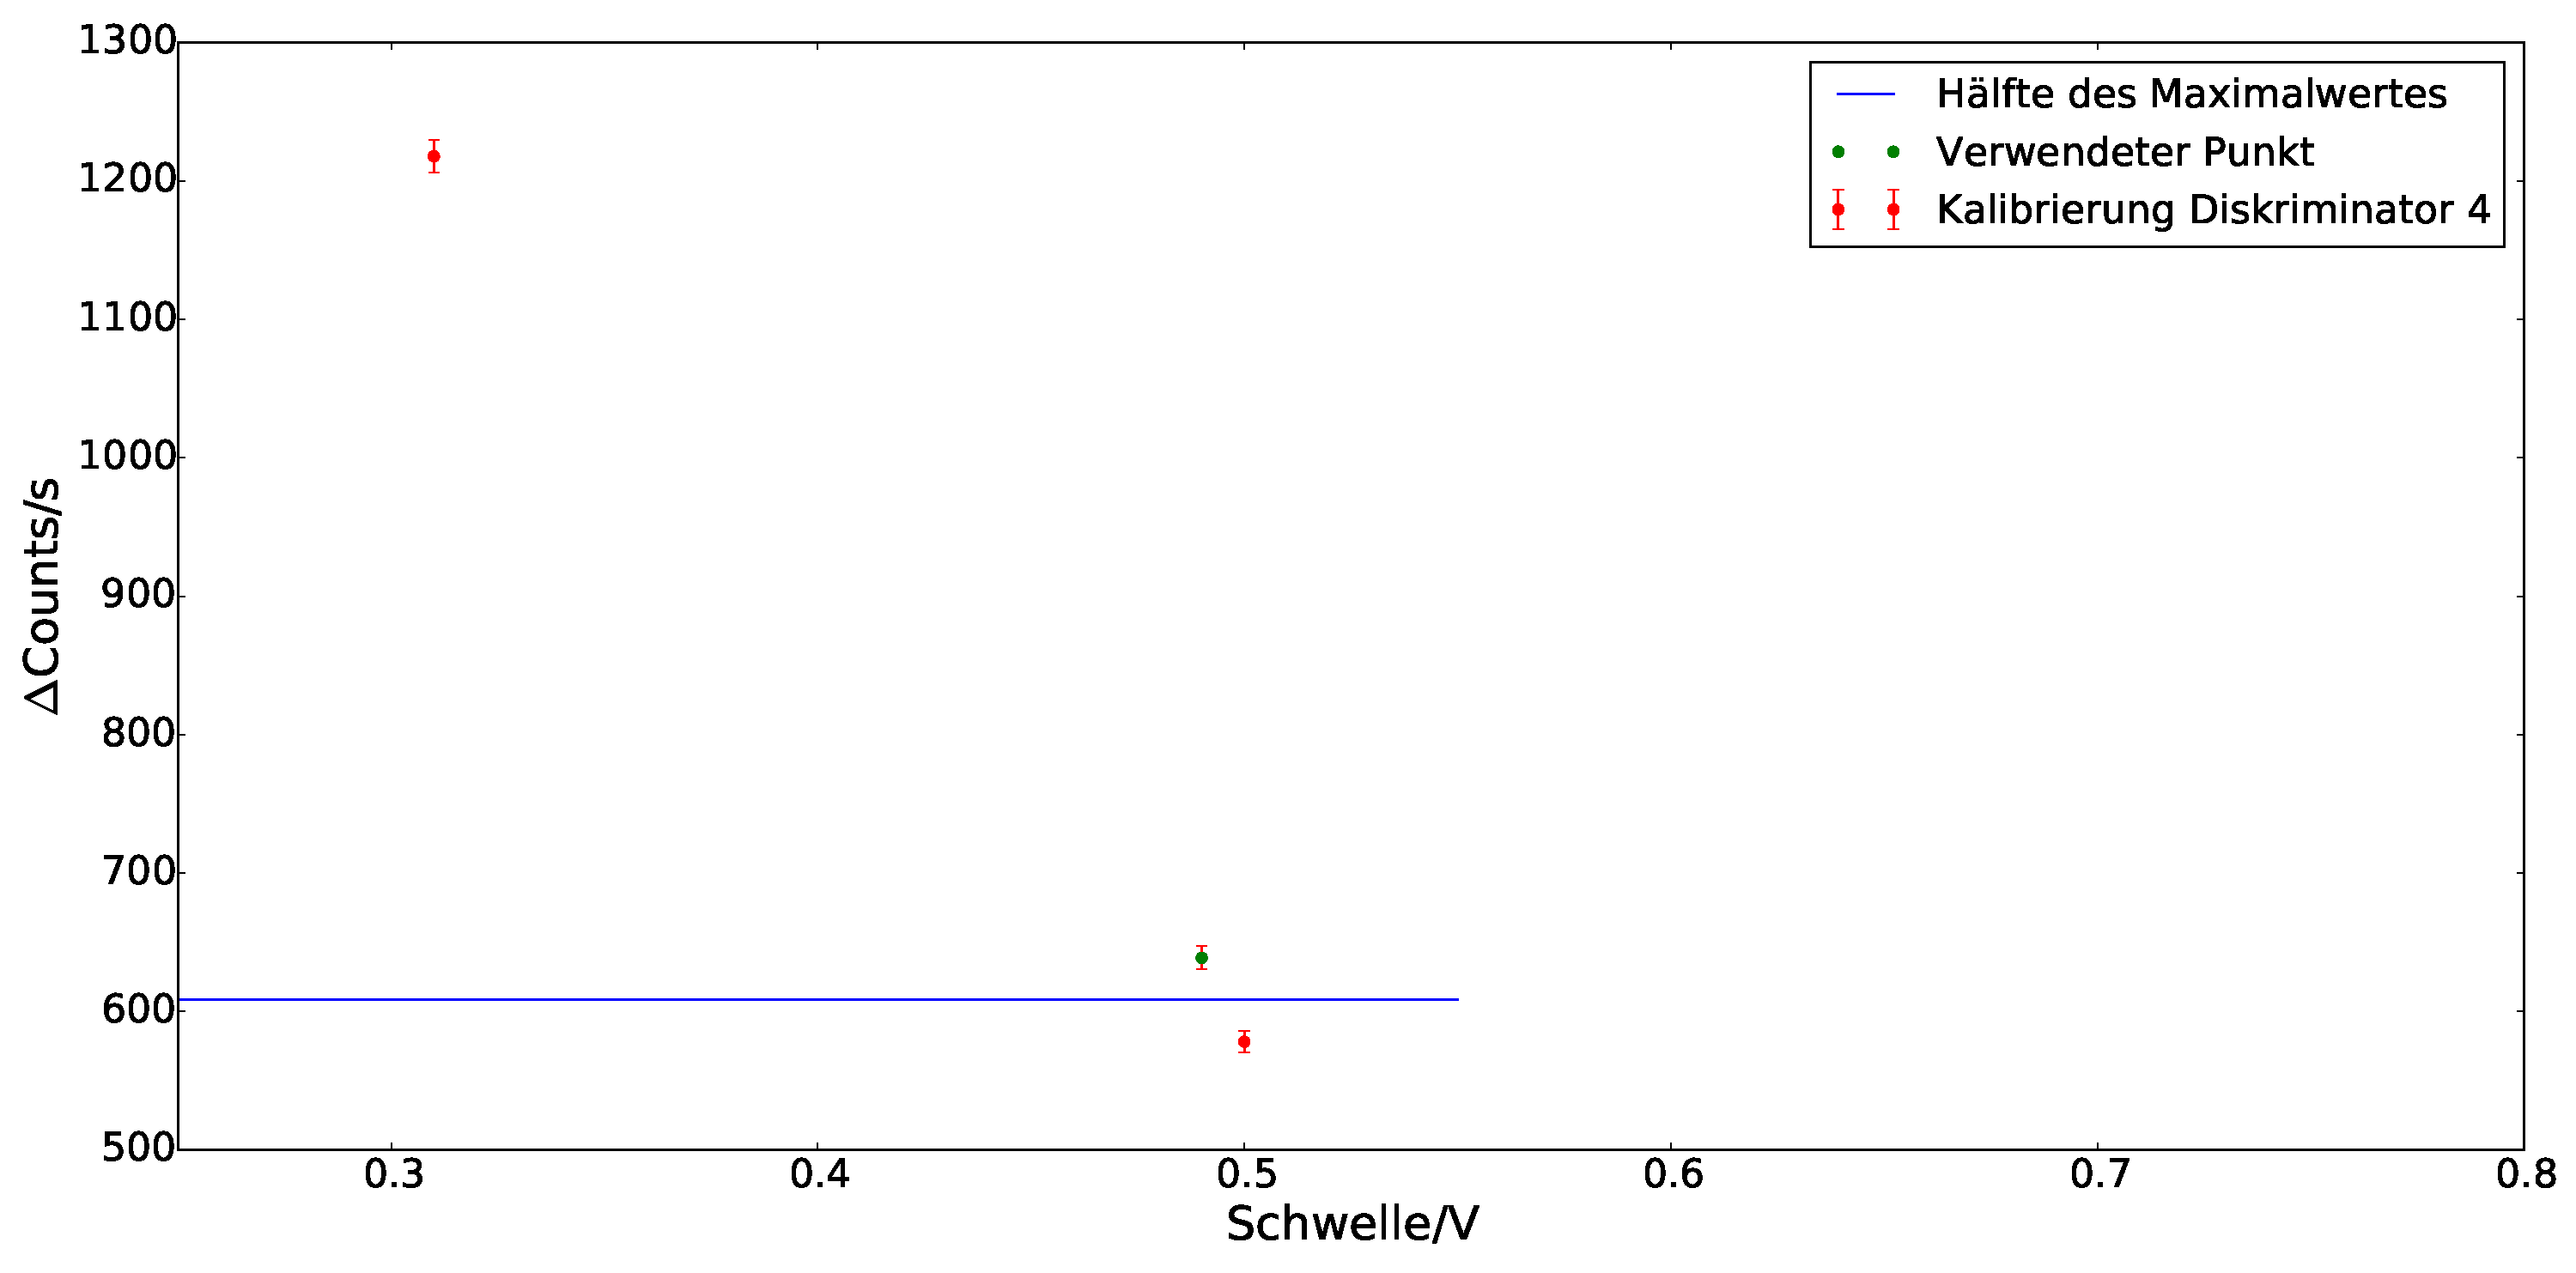
\includegraphics[scale = 0.35]{Disk_4.pdf}
\caption{Differenzplot der Counts gegen die Schwellspannung f�r Diskriminator 4}
\label{fig:Disk_4}
\end{figure}
Die Energien der Photonen beim Zerfall von $^{60}$Co werden in Abb. \ref{fig:Co_60} dargestellt.(vgl. \cite{Co_60})
\begin{figure}[H]
\centering
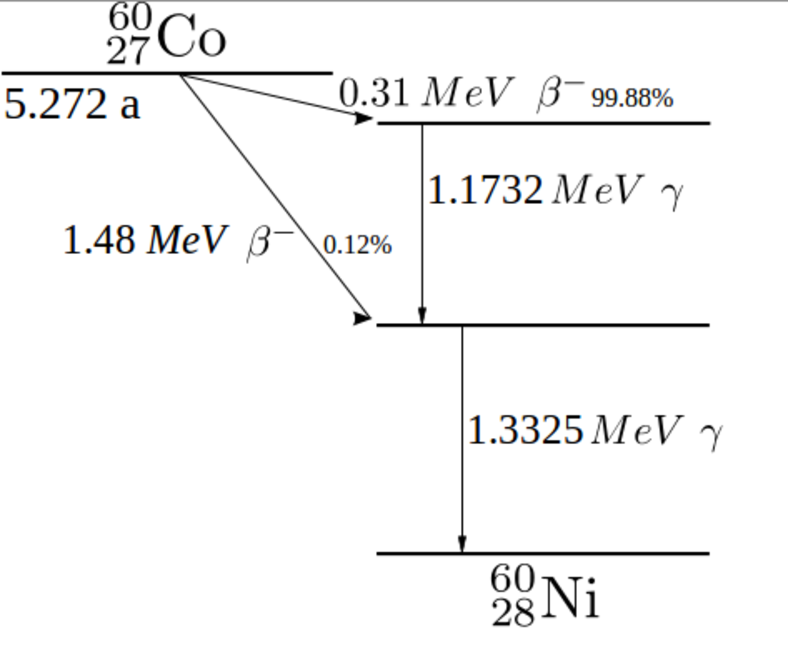
\includegraphics[trim = 0cm 0cm 0cm 1.1nm,scale = 0.5, clip]{Cobalt60_Zerfall.pdf}
\caption{Zerfall von $^{60}$Co}
\label{fig:Co_60}
\end{figure}
In Tabelle \ref{tab:Schwellwerte} sind die Diskriminatorschwellen f�r Diskriminator 1 bis 4 aufgelistet.
\begin{table}[H]
\caption{Diskriminatorschwellwerte}
\begin{tabular}{c|c|c|c|c|}
 & Diskriminator 1 & Diskriminator 2 & Diskriminator 3 & Diskriminator 4 \\ 
\hline Untere Schwelle & 0,70 V & 0,51 V & 0,41 V & 0,49 V \\ 
\hline Obere Schwelle &  &  & 0,52 V &  \\ 
\hline 
\end{tabular}
\label{tab:Schwellwerte}
\end{table}
\subsection{Delay}
Da PM1, PM2 und PM4 �ber eine logische Einheit verbunden sind, welche den TAC startet, muss sichergestellt werden, dass die Signale der drei Photomuliplier Zeitgleich ankommen. Die Zeitversetzung (Delay) der Signale wird �ber die Kabell�nge der Photomuliplier zur logischen Einheit eingestellt.

Es kann angenommen werden, das die Signale von PM3 und PM4 zur selben Zeit ankommen. Deshalb kann das Signal von PM3 gut als Referenz f�r die ersten beiden verwendet werden. F�r die Bestimmung des Delays werden PM1 (bzw. PM2) und PM3 an die logische Einheit angeschlossen, jedoch ohne ein Veto. Die Szintillatoren werden so geschaltet, dass nur bei gleichzeitigem Signal hochgez�hlt wird. Es wird erwartet, das sich ein Plateau ausbildet. Der Delay in der Mitte des Plateaus ist die optimale Einstellung, das sich die Signale an diesem Punkt �berlagern. Damit sich ein m�glichst schmales Plateau ausbildet, m�ssen die Pulse der Diskriminatoren kurz sein. In Abbildung \ref{fig:delay_1} ist zu sehen, dass f�r den ersten Photomulipier kein eindeutiges Plateau identifiziert werden konnte. Deshalb musste das Delay mit dem Oszilloskop eingestellt werden, um sicherzustellen, dass sich die beiden Signale �berlappen. F�r den ersten Photomuliplier wurde mit dem Oszilloskop ein Delay von 9ns bestimmt. In Abbildung \ref{fig:delay_2} sind die Messdaten f�r den zweiten Photomuliplier zu sehen. Im Bereich von 20 bis 28ns ist ein Plateau zu erkennen, das Delay wurde mit dem Wert (24ns) in der Mitte des Plateaus angenommen. Das Delay von 24ns f�r den zweiten Photomuliplier wurde zus�tzlich mit dem Oszilloskop bestimmt und konnte best�tigt werden.

\begin{figure}[H]
	\centering
  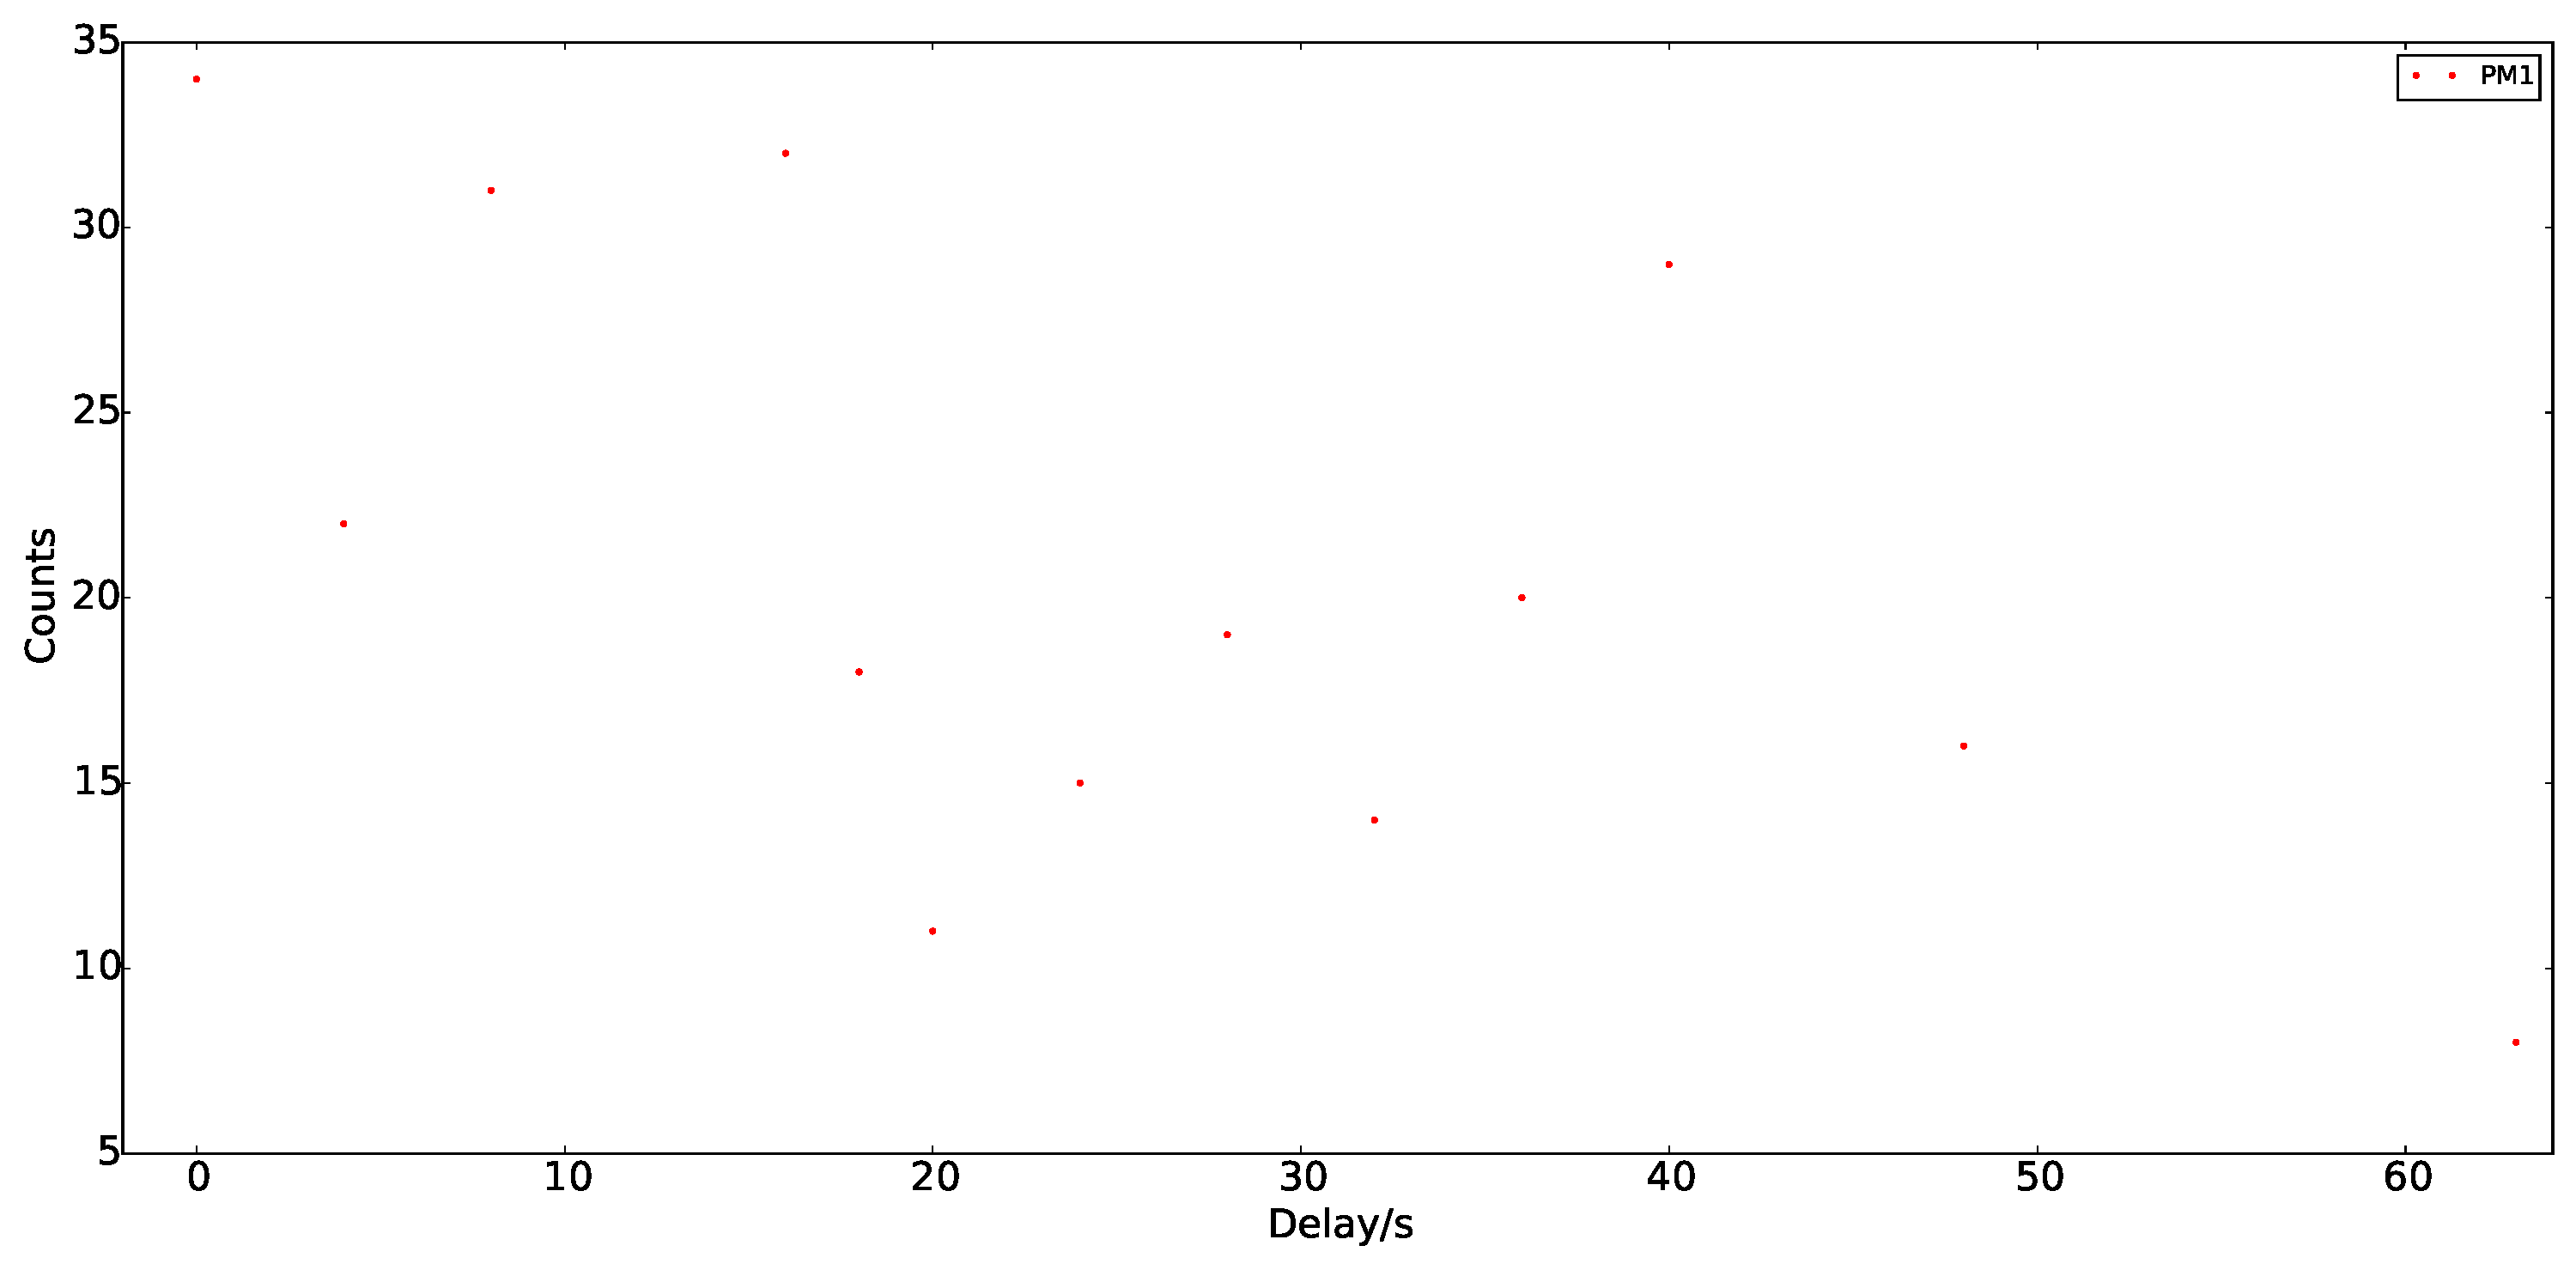
\includegraphics[scale=0.33]{delay_1.pdf}
	\caption{Counts in Abh�ngigkeit vom Delay f�r die ersten Photomuliplier, es ist kein eindeutiges Plateau zu erkennen. Deshalb wurde das Signal mit einem Oszilloskop betrachtet und ein Delay von 9ns bestimmt.}
	\label{fig:delay_1}
\end{figure}


\begin{figure}[H]
	\centering
  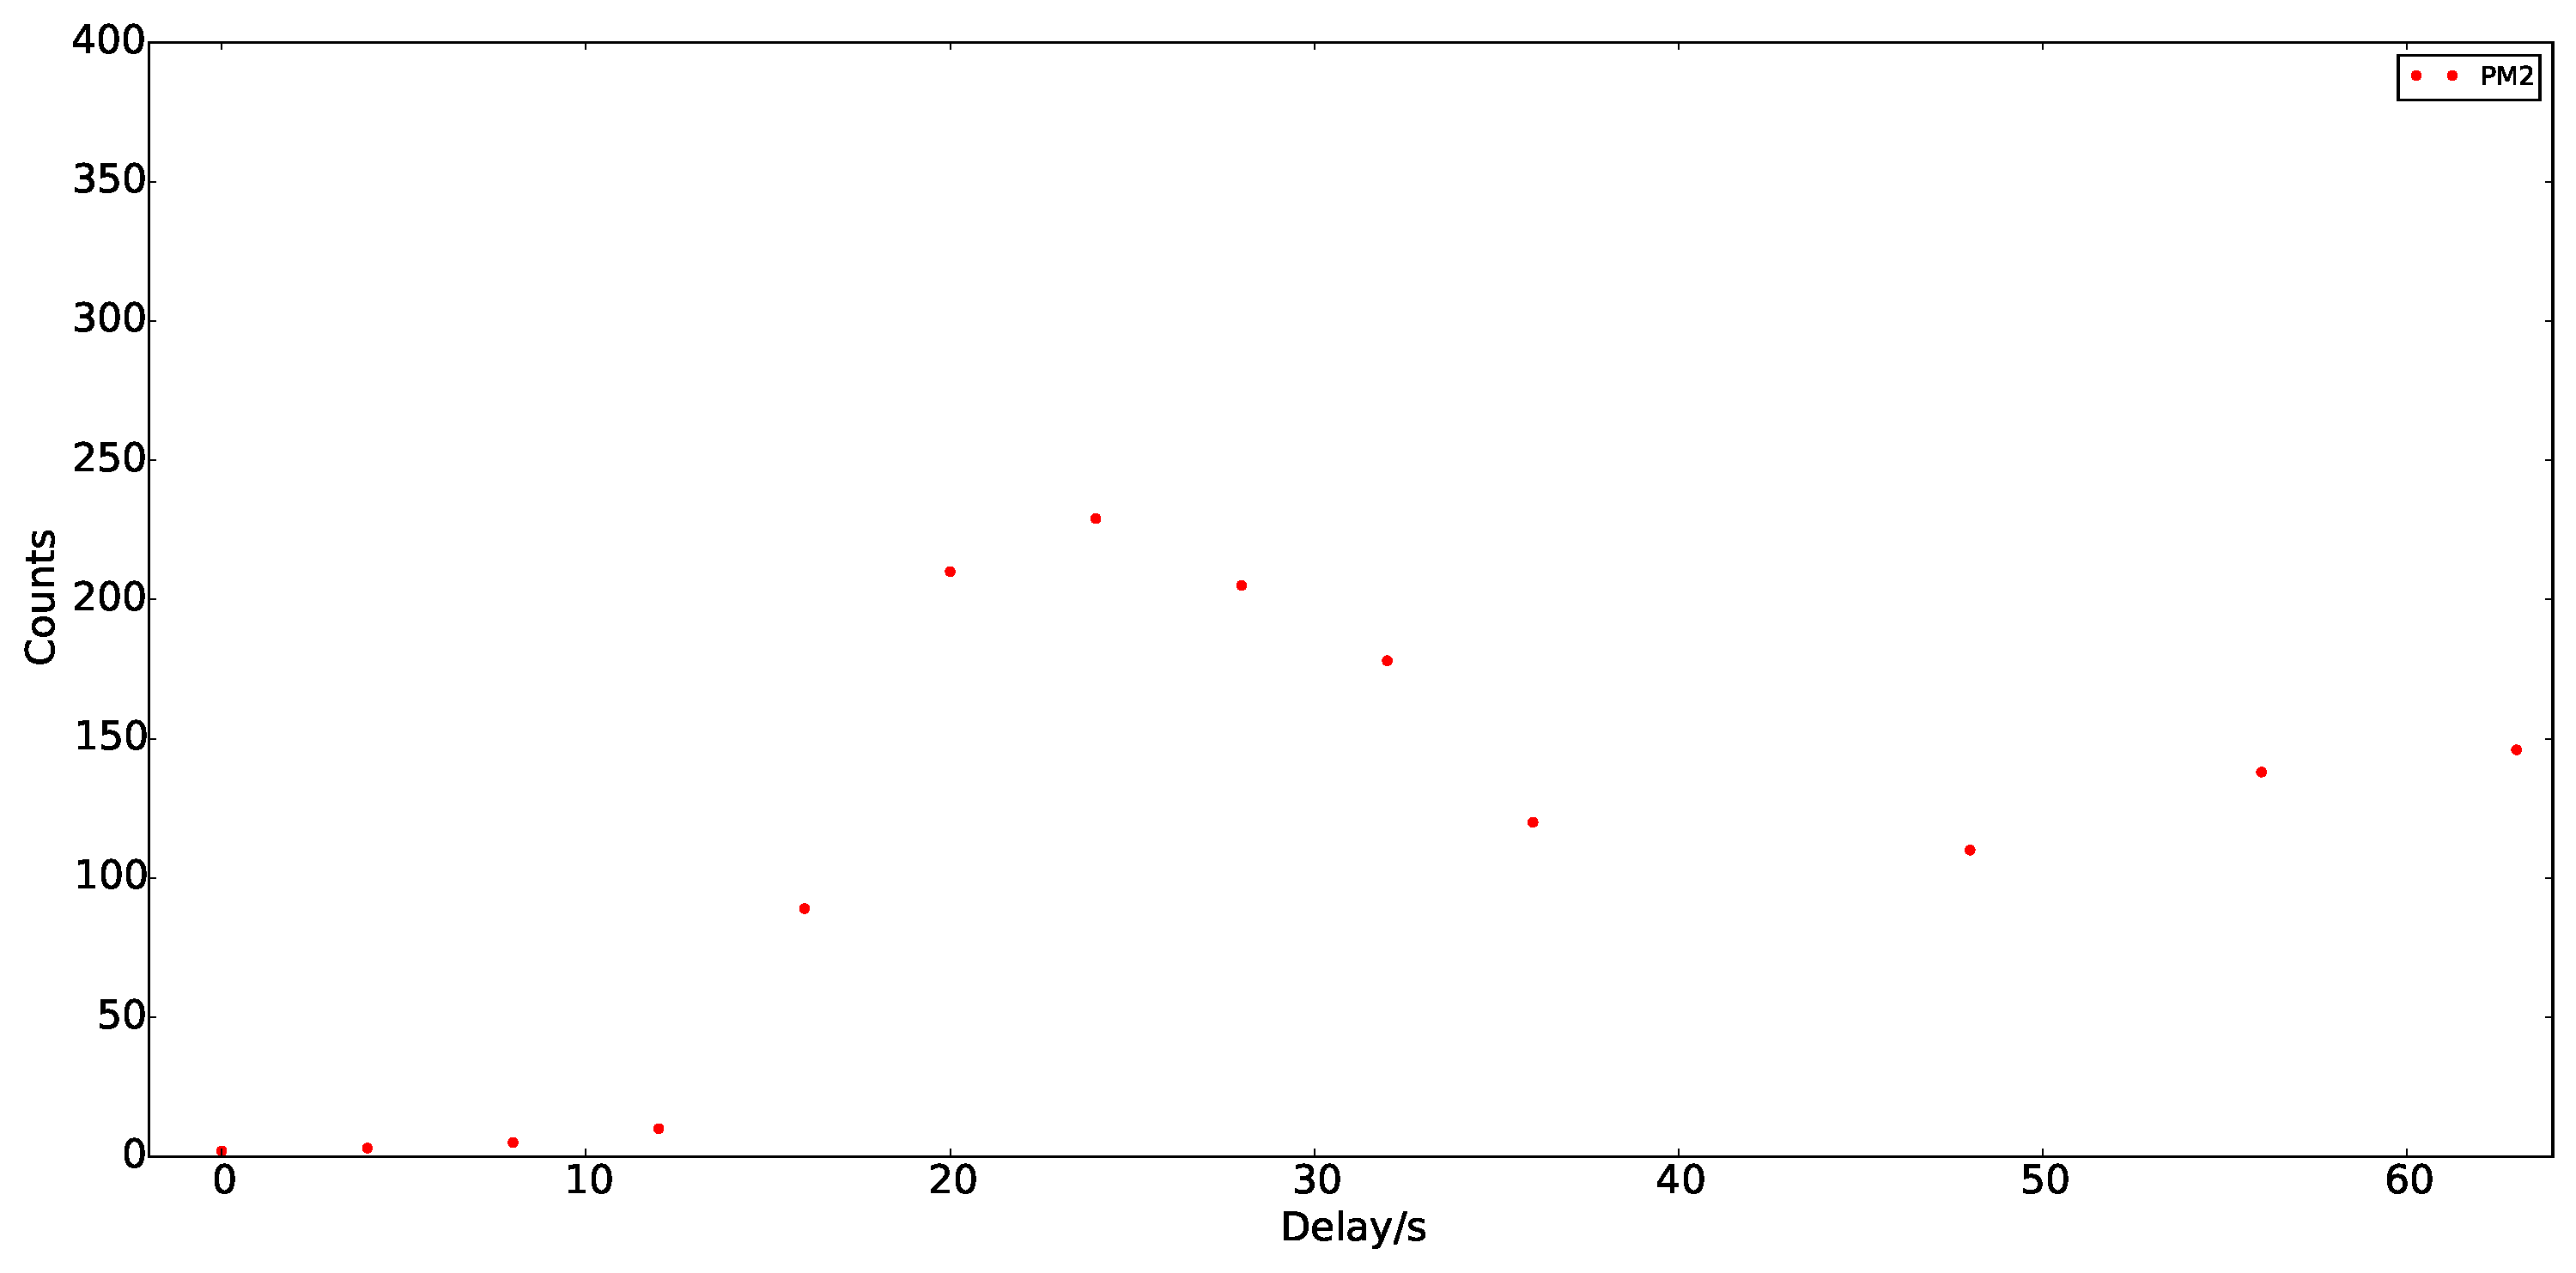
\includegraphics[scale=0.33]{delay_2.pdf}
		\caption{Counts in Abh�ngigkeit vom Delay f�r die ersten Photomuliplier. Ein Plateau ist im Bereich von 20 bis 28 ns zu erkennen. Das Delay wurde mit 24 ns, in der Mitte des Plateaus bestimmt. dieser Wert wurde mit dem Oszilloskop verifiziert.}
	\label{fig:delay_2}
\end{figure}

Es ergeben sich die Delays in Tabelle \ref{tab:delay}.

\begin{table}[H]
	\centering
	\caption{Optimal bestimmtes Delay f�r PM1 und PM2}
	\label{tab:delay}
	\begin{tabular}{|c|c|}
	\hline Photomuliplier & Delay [ns] \\ \hline
	\hline PM1 & 9 \\ 
	\hline PM2 & 24 \\ 
	\hline 
	\end{tabular} 
\end{table}

Das Oszilloskopbild Abb. \ref{PMT2Delay} zeigt, dass die Signale beim zweiten Photomultiplier �bereinander liegen. Auff�llig war, dass trotz Abschlusswiderstand verschobene Signale angezeigt wurden, die eigentlich nicht zu sehen sein sollten.
\begin{figure}[H]
\centering
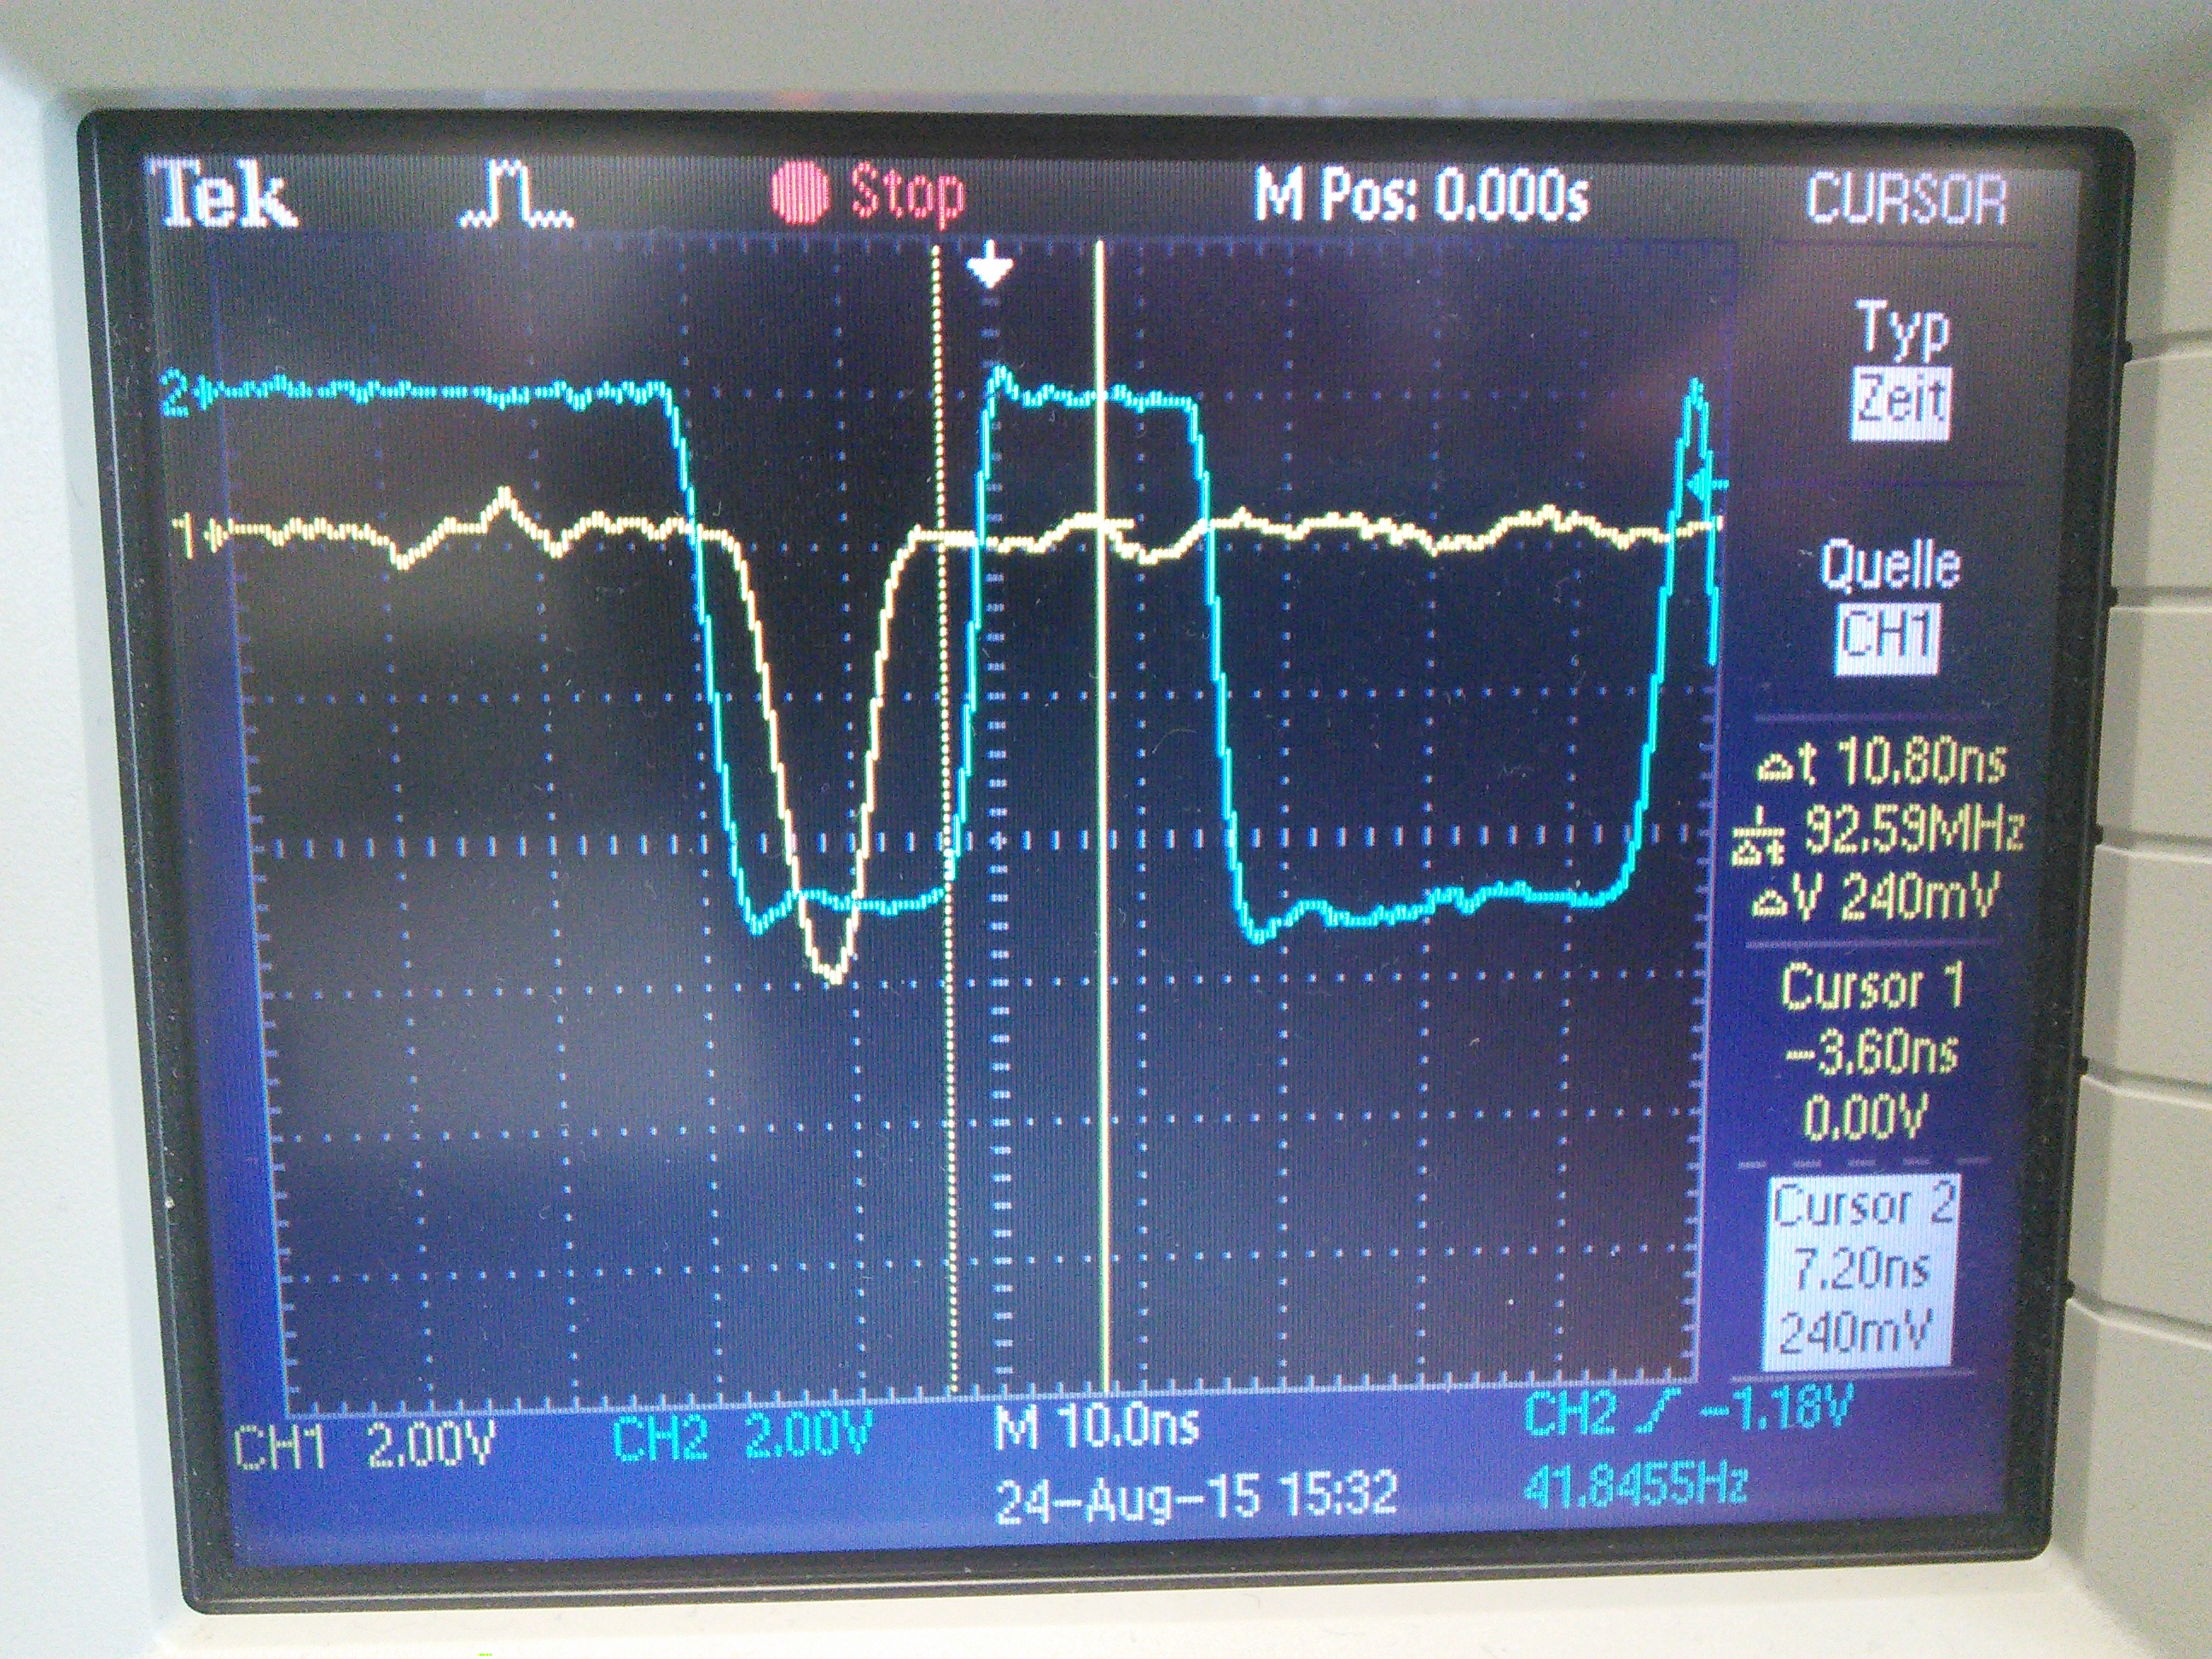
\includegraphics[scale=0.12]{DelayPMT2}
\caption{Oszilloskopbild Delay PMT 2}
\label{PMT2Delay}
\end{figure}
\subsection{Kanal-Zeit-Eichung}
F�r eine genaue Bestimmung der Lebensdauer von Myonen ist eine exakte Zeiteichung extrem wichtig. F�r die Zeiteichung wird ein TAC, ein dual Timer und ein Oszilloskop verwendet. Der schematische Aufbau ist in Abbildung \ref{fig:kanal_zeit} zu sehen. 

\begin{figure}[H] 
	\centering
  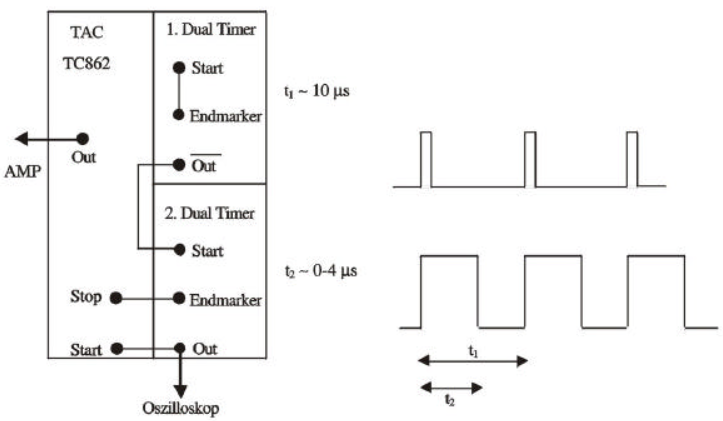
\includegraphics[scale=0.5]{kanal_zeit.png} 
	\caption{Schematischer Aufbau f�r die Kanal-Zeit-Eichung}
	\label{fig:kanal_zeit}
\end{figure}

Der dual Timer wird verwendet, um kurze Signale mit bekannter L�nge zu erzeugen. �ber die High und Lows des Signals wird der TAC gesteuert, wodurch eine Spannung in Abh�ngigkeit der L�nge des Signals erzeugt wird. Das Signal wird verst�rkt und mit dem ADC digitalisiert, damit es vom Mulit-Channel-Analyser verwertet werden kann. Durch variiren der Signall�nge lassen sich die verschiedene Kan�le ansprechen, wodurch eine Beziehung zwischen einer Zeit und einem Kanal hergestellt wird. Die Zeitintervalle werden gegen die Kan�le aufgetragen und mit Gleichung \ref{eqn:kanal} gefittet. Zum Vergleich soll zus�tzlich ein Fit mit $B = 0$ erzwungen werden. Die Parameter und Variablen des Fits sind in Tabelle \ref{tab:fit_kanal} zu sehen

\begin{align}
\label{eqn:kanal}
t = A*k+B
\end{align}

\begin{table}[H]
	\caption{Parameter des Fits}
	\label{tab:fit_kanal}
	\begin{tabular}{c|l}
	t & Zeitintervall in $\mu$s \\ 
	k & Kanal \\ 
	A & Proportionalit�tsfaktor \\ 
	B & Offset \\ 
	\end{tabular} 
\end{table}

In Abbildung \ref{fig:kanal_zeit_fit} sind die Messwerte zu sehen. F�r die Fitparameter ergaben sich dabei die Werte in Tabelle \ref{tab:fit}. Das $\chi_{red}^2$ hat ein Wert von 0,02, was einem guten Fit entspricht.

\begin{table}[H]
\centering
\caption{Fitparameter mit Fehlern und $\chi_{red}^2$}
\label{tab:fit}
\begin{tabular}{|c|c|}
\hline Paramter & Wert \\ 
\hline A & 0,002106(6) \\ 
\hline B & 0,126(19) \\ 
\hline $\chi_{red}^2$ & 0,233 \\ 
\hline 
\end{tabular} 
\end{table}

\begin{figure}[H] 
	\centering
	  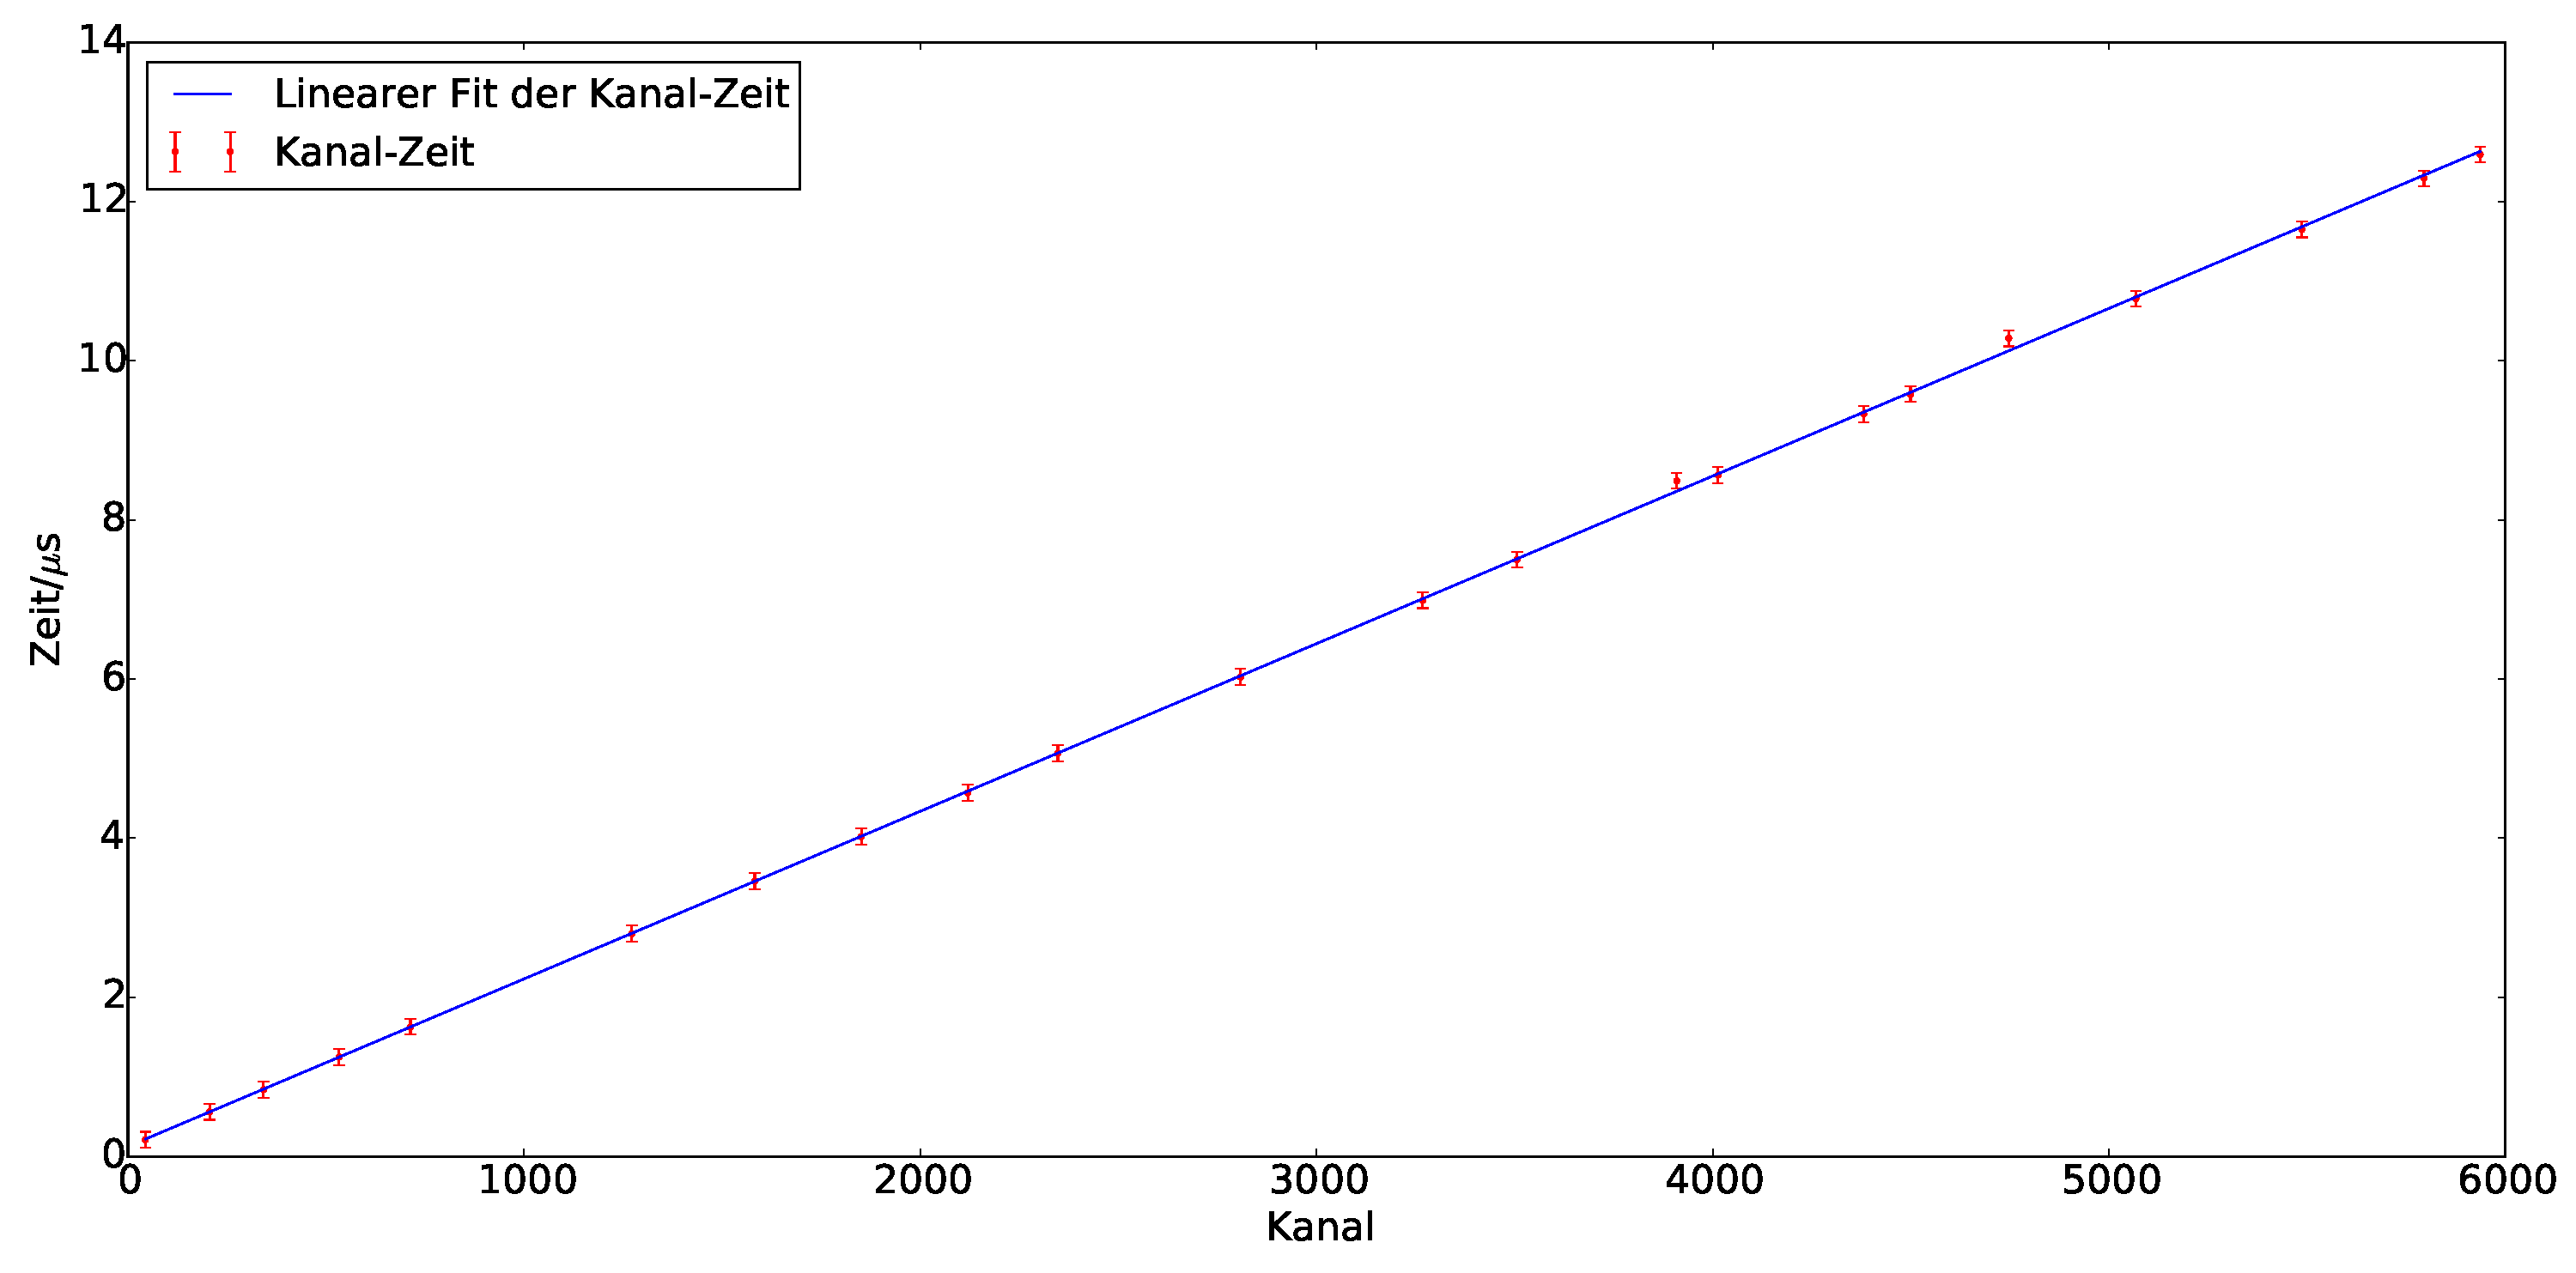
\includegraphics[scale=0.33]{kanal_zeitax+b.pdf} 
	\caption{Kanal-Zeit-Eichung}
	\label{fig:kanal_zeit_fit}
\end{figure}
Zum Vergleich sind die Fitparameter f�r $B = 0$ in Tabelle \ref{tab:fit2} zu sehen. Der Fit f�r $B = 0$ ist in Abb. \ref{fig:kanal_zeit_fit2} dargestellt.
\begin{table}[H]
\centering
\caption{Fitparameter mit Fehlern und $\chi_{red}^2$ f�r $B = 0$}
\label{tab:fit2}
\begin{tabular}{|c|c|}
\hline Paramter & Wert \\ 
\hline A & 0.002136(5) \\ 
\hline B & 0 \\ 
\hline $\chi_{red}^2$ & 0,719 \\ 
\hline 
\end{tabular} 
\end{table}
\begin{figure}[H] 
	\centering
	  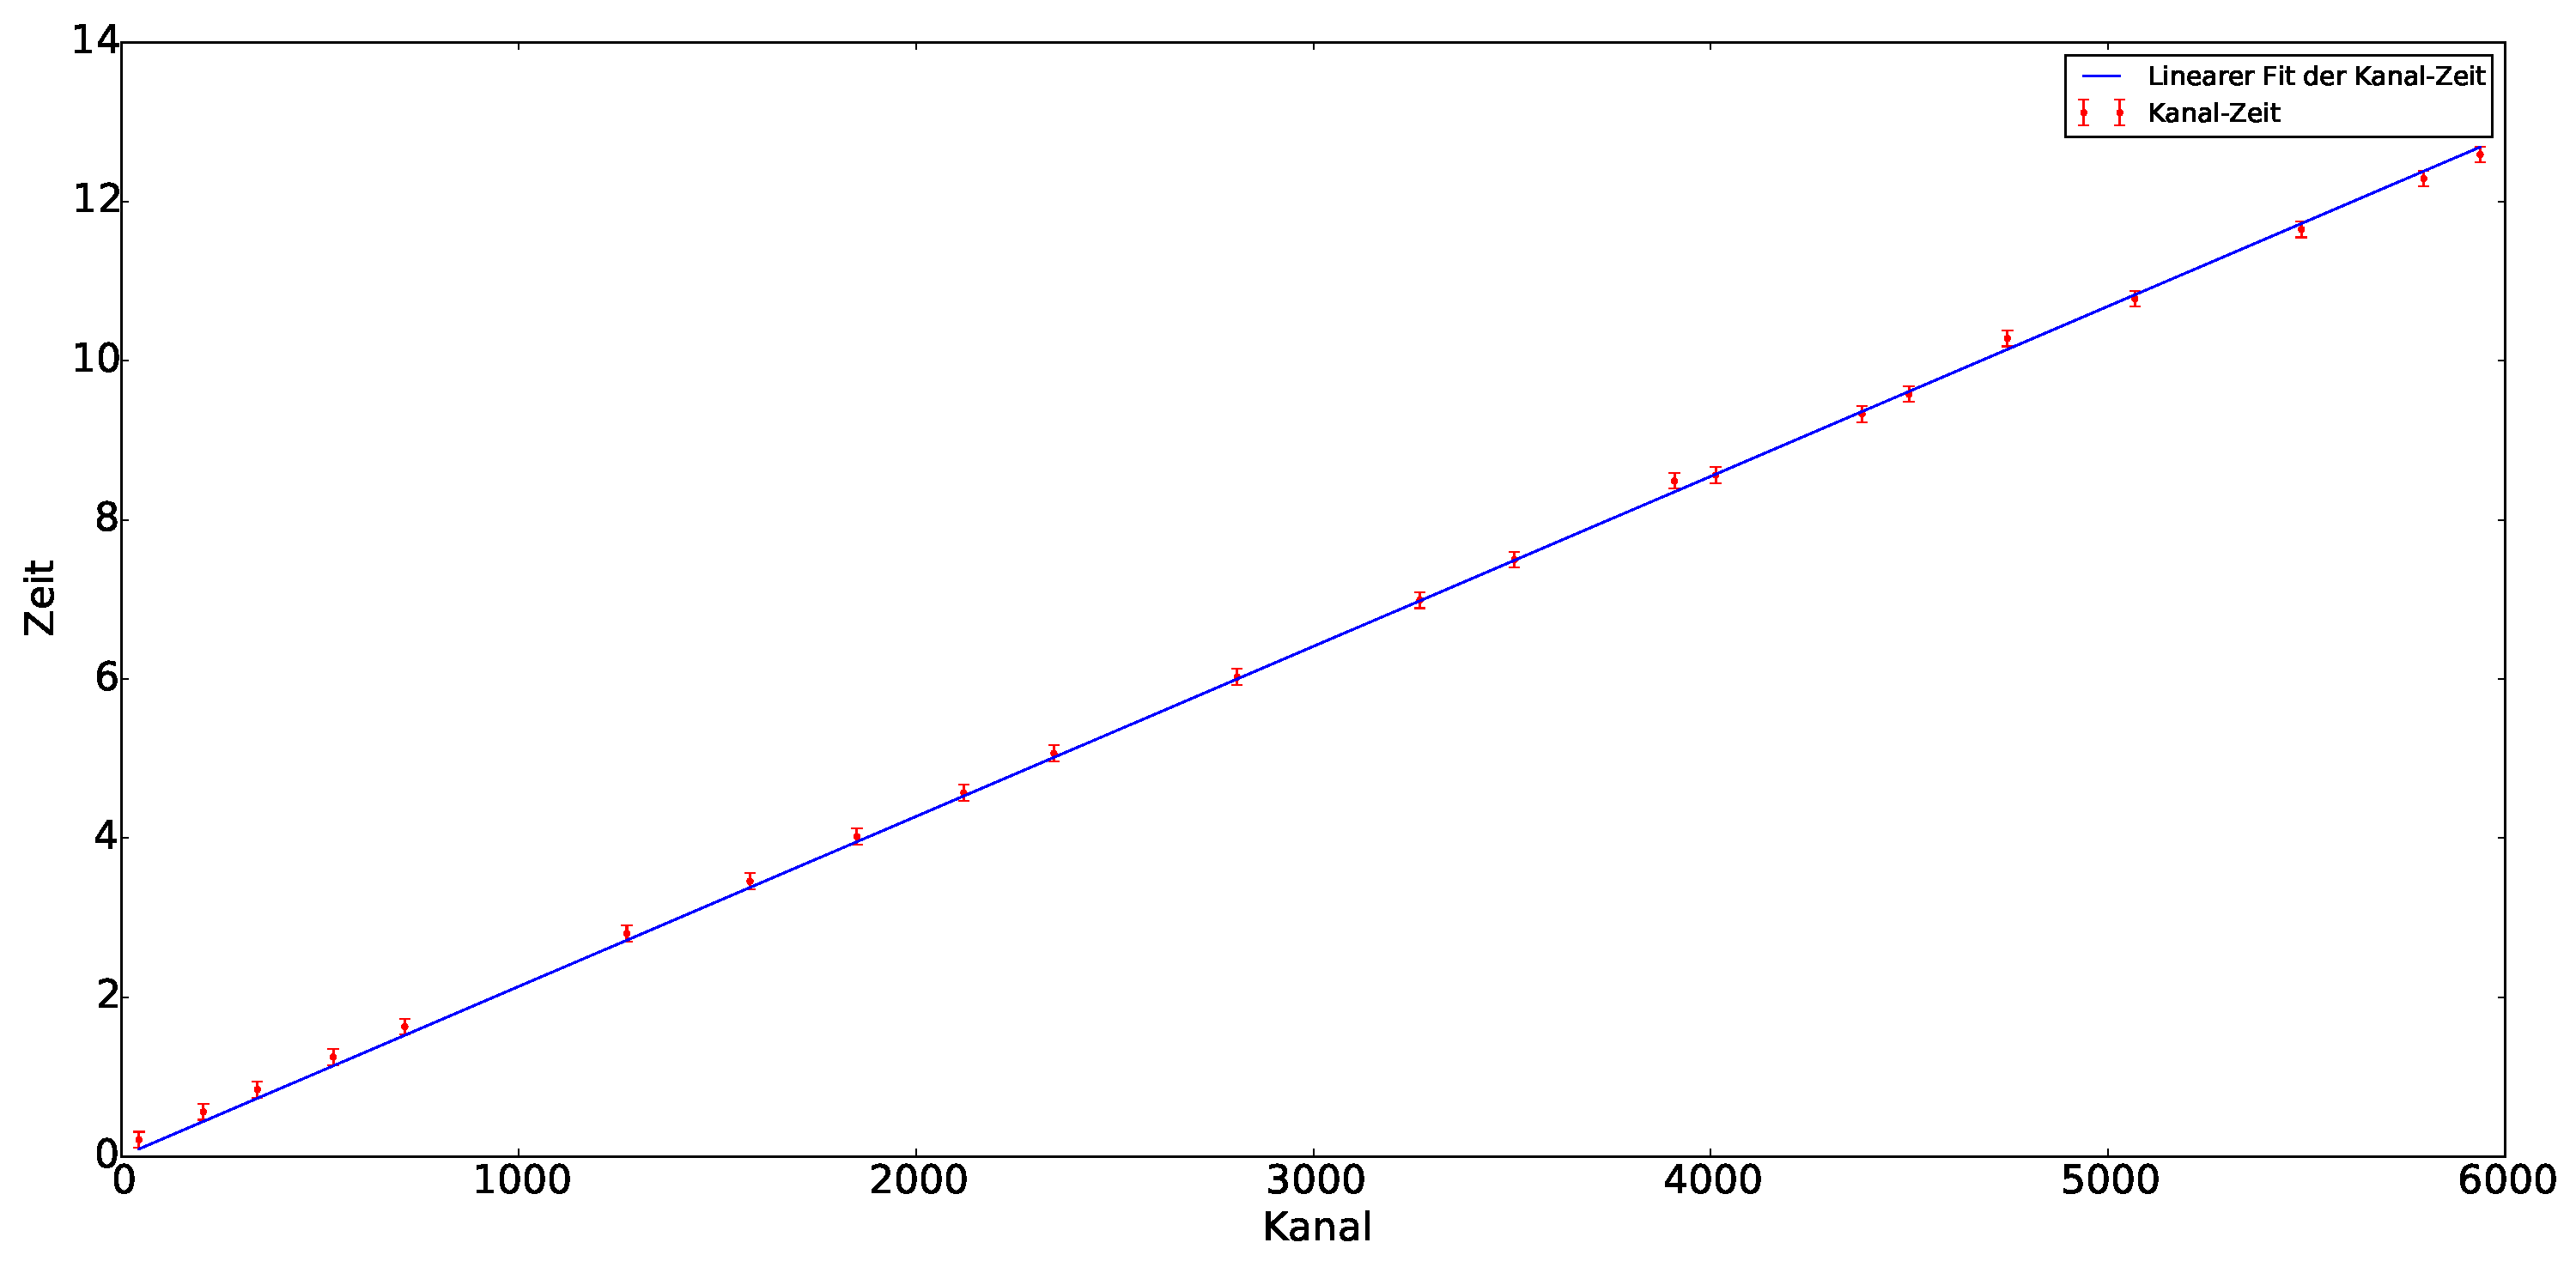
\includegraphics[scale=0.33]{kanal_zeitax.pdf} 
	\caption{Kanal-Zeit-Eichung f�r $B = 0$}
	\label{fig:kanal_zeit_fit2}
\end{figure}
\subsection{Messung der mittleren Lebensdauer}
Nachdem die umfangreichen Kalibrationen beendet sind, soll die Lebensdauer der Myonen anhand der Messdaten bestimmt werden. Dazu werden die folgenden Methoden verwendet und deren Resultat verglichen.
\subsubsection{Maximum Likelihood Methode}
Um die mittlere Lebensdauer von Myonen zu bestimmen eignet sich die Maximum Likelihood Methode. Wie in Abschnitt 2.3 besprochen sind Zerfallszeiten mit Zeitunabh�ngiger Zerfallsrate exponentialverteilt, sodass sich die einparametrige Warscheinlichkeitsdichte
\begin{align}
P(t_i|\tau) = \frac{1}{\tau}\frac{e^{-\frac{t_i}{\tau}}}{e^{-\frac{T_1}{\tau}}-e^{-\frac{T_2}{\tau}}}
\end{align}
ergibt. Da die Messung des Zeitintervalls nach oben und unten beschr�nkt ist, wurde die Warschenlichkeitsdichte normiert, wobei $T_1$ die untere Schranke und $T_2$ die obere Schranke der Zeitmessung ist. Es wird davon ausgegangen, dass die einzelnen Zeitmessungen unabh�ngig voneinander sind, sodass sich f�r die gesamte Messung die n-dimensionale Warscheinlichkeitsdichte
\begin{align}
L = \prod_{i=1}^N P(t_i|\tau) = \prod_{i=1}^N \frac{1}{\tau}\frac{e^{-\frac{t_i}{\tau}}}{e^{-\frac{T_1}{\tau}}-e^{-\frac{T_2}{\tau}}}
\end{align}
ergibt. Es wird davon ausgegangen, dass die gemessenen Zerfallszeiten der wahrscheinlichsten Messung entsprechen, sodass die Messung einem Maximum der Warscheinlichkeitsdichtefunktion bez�glich $\tau$ entspricht. Um das Maximum von $L$ zu bestimmen betrachtet man die Funktion
\begin{align}
\ln{L} = \ln\left[\prod_{i=1}^N P(t_i|\tau)\right] = \sum_{i=1}^{N}\ln[P(t_i|\tau)] = -\left[\sum_{i=1}^{N}\ln(\tau) + \frac{t_i}{\tau} + \ln(e^{-\frac{T_1}{\tau}}-e^{-\frac{T_2}{\tau}})\right]
\end{align}
und bestimmt die Nullstelle der Ableitung nach $\tau$.
Schlie�lich erh�lt man die beste Approximation f�r die Lebensdauer $\tau$:
\begin{align}
\hat{\tau} = \frac{1}{N}\sum_{i=1}^{N} t_i - \frac{T_1e^{-\frac{T_1}{\tau}}-T_2e^{-\frac{T_2}{\tau}}}{e^{-\frac{T_1}{\tau}}-e^{-\frac{T_2}{\tau}}}
\end{align}
Da es nur M Kan�le und damit M m�gliche Zeiten $t_k$ gibt, kann die erste Summe umgeschrieben werden,
\begin{align}
\sum_{i=1}^{N} t_i = \sum_{k=1}^{M} N_k t_k \text{ wobei } N = \sum_{k=1}^{M} N_k
\end{align}
sodass der Fehler von $\hat{\tau}$ �ber den statistischen Fehler auf $N_k$, welcher $\sqrt{N_k}$ betr�gt, bestimmt werden kann.
Es ergibt sich also
\begin{align}
\hat{\tau} = \sum_{k=1}^{M} N_k t_k - \frac{T_1e^{-\frac{T_1}{\tau}}-T_2e^{-\frac{T_2}{\tau}}}{e^{-\frac{T_1}{\tau}}-e^{-\frac{T_2}{\tau}}}
\end{align}
mit einem Fehler von
\begin{align}
\Delta\hat{\tau} = \frac{1}{N}\sqrt{\sum_{k=1}^{M}N_kt_k^2}
\end{align}


